\documentclass[12pt]{article}
% \usepackage{scrtime} 
\usepackage{booktabs}
\usepackage{tabularx}
\usepackage{pdflscape}
\usepackage{array}
\usepackage[margin=1in]{geometry}
\usepackage{hyperref}
\usepackage{graphicx}
\usepackage{amsmath} 
\usepackage{caption}
\usepackage{subcaption}
\usepackage[backend=biber,style=vancouver,sortcites=true]{biblatex}
\addbibresource{ms2.bib}
\usepackage{multirow} 
\usepackage{graphicx} % Required for inserting images
\usepackage{cleveref}
\usepackage{titlesec}
\usepackage[section]{placeins}
\usepackage{float}

\usepackage{listings}
\usepackage{xcolor}

\lstset{
    language=Python,
    basicstyle=\ttfamily\small,
    keywordstyle=\color{blue},
    stringstyle=\color{orange},
    commentstyle=\color{gray},
    showstringspaces=false,
    breaklines=true,
    frame=single
}

% Short title (<=70 characters) -- enter in submission system running header field
\newcommand{\shorttitle}{Evaluation of Automated Historical Disease-Surveillance Extraction}

\title{Evaluation of automated table extraction for historical infectious-disease surveillance data}

% NOTE FOR AUTHORS -- before submission: add ORCID iDs for all authors in the
% Editorial Manager submission system (not supplied here; verify with each author).
\author{
  Eden Ofek Nalian\textsuperscript{1} \and
  Steven C.\ Walker\textsuperscript{1} \and
  David J.\,D.\ Earn\textsuperscript{1} 
}
%%\date{August 2025}
\date{\today}

%%% PLOS submission: line numbers + double spacing %%%
\usepackage{lineno}
\linenumbers
\usepackage{setspace}
\doublespacing
%%%%%%%%%%%%%%%%%%%%%%%%%%%%%%%%%%%%%%%%%%%%%%%%%%%%%%

\begin{document}

\maketitle

\begin{center}
\small
\textsuperscript{1}Department of Mathematics \& Statistics, McMaster University, Hamilton, Ontario, Canada \\

Corresponding author: eden.nalian@gmail.com (Eden Ofek Nalian)

\end{center}




\begin{abstract}
The majority of historical epidemiological data remains undigitized. This paper evaluates the effectiveness of automated table extraction as an alternative to manual data entry. We assess the performance of \emph{Amazon Textract} on a large dataset of historical infectious disease records, comparing extraction accuracy, error characteristics, and overall efficiency against traditional manual transcription methods. Cell-level agreement was evaluated on the 1956 tables (53{,}872 evaluated cells), where content-only agreement between the automated and manually transcribed data was 88.5\% overall and 92.9\% among cells that were numeric in the manual reference transcription (a secondary figure of 95.6\% obtains if the denominator is instead restricted to cells numeric on both sides); downstream epidemiological comparisons (disease peaks, growth rates, and cross-correlations) span all three years of the dataset, 1956--1958. Most residual cell mismatches had a Levenshtein distance of one or two; larger discrepancies were concentrated in rows affected by disease-name or row-alignment failures, and differences in the selected downstream epidemiological summaries were generally modest. Extraction runtime was short relative to an extrapolated manual-entry estimate, but total person-time, including post-processing, was not measured. As well, the measured post-processing time we did record was a small proportion of the total time previously required for the whole task. Overall, this paper illustrates the potential and limitations of a human-in-the-loop workflow for transforming historical tabular data of this kind into digital formats.
\end{abstract}

\section{Introduction} \label{sec:intro}

Weekly notifiable-disease reports have been collected in printed form for well over a century, but the overwhelming majority remain undigitized and therefore unavailable for computational analysis. Where such records have been converted to machine-readable form, this has typically been achieved by manual transcription -- a process that is accurate but slow enough to constrain which archives are digitized at all, and which is not itself error-free (\cref{sec:NDD} documents an instance in which the manual transcription used in this study contained an error that the automated extraction did not). Automated table extraction offers an obvious alternative, but for a researcher who intends to fit models to the resulting series, the relevant question is not how well a tool reads cells in the abstract. It is whether the epidemiological quantities computed from the extracted data match those computed from a trusted transcription, and, where they do not, whether the discrepancies can be detected without one.

Much work has been done on software that converts images of tables into machine-readable data, such as comma-separated value (CSV) files. The problems such software addresses are typically decomposed into distinct tasks, though different authors characterize them differently \cite{zhong2020image}. We organize our work around three tasks:
\begin{description}
    \item[Table detection:] Locating tables in documents.
    \item[Table structure recognition:] Parsing the row and column layout of tables.
    \item[Content recognition:] Identifying the content of table cells and headers.
\end{description}
Table detection and layout are surprisingly difficult tasks for computers given how easy they are for humans \cite{hu2002evaluating}, a difficulty with roots in decades of OCR research \cite{Mori1992} and still evident in widely used open-source engines such as Tesseract \cite{TessOverview}. Modern document-AI systems -- including large vision-language models applied directly to spreadsheets and tables -- continue to report substantial failure modes on structurally irregular inputs even on contemporary, cleanly scanned material \cite{xia2024vision,Sahasrabudhe2025}, a limitation that only compounds on historical documents, where period typography, physical degradation, and non-standard layouts are the norm rather than the exception. Software that actively produces usable results, in the sense of data similar enough to the scanned document to support similar downstream conclusions, must succeed at all three tasks at least reasonably well; a single under-performing sub-task is often enough to compromise the result, as we discuss in \cref{sec:NDD}.

Historical health-surveillance archives are a natural and comparatively under-served target for this technology. Project Tycho is the most developed prior effort of this kind, digitizing over a century of United States notifiable-disease reports \cite{van2013contagious,van2018project}; Canada's own notifiable-disease surveillance system has a comparably long paper record that has, until recently, remained largely undigitized \cite{sockett1996communicable,totten2019updates}. What is largely absent from this literature, and from table-extraction benchmarks generally, is evaluation against an independent transcription with downstream, analysis-level epidemiological quantities -- not only cell-level accuracy -- as the endpoint. Benchmark accuracy on curated corpora does not say whether the peak timing, growth rate, or cross-correlation an epidemiologist computes from an extracted series would match what they would compute from a trusted transcription, or whether the discrepancies could be caught without one. Reference transcriptions are also conventionally treated as an infallible standard against which extraction is scored; in fact, as we show in \cref{sec:NDD}, they can themselves contain errors that a careful comparison can surface.

Using 156 weekly tables from the Canadian Disease Incidence Dataset (CANDID; 1956--1958) \cite{CANDID}, we ask: how closely does a documented, staged Textract-based extraction and post-processing workflow reproduce an independently produced manual transcription at the cell level (evaluated here for the 1956 tables); which classes of error survive each processing stage; and how well are standard epidemiological summaries -- peak timing, peak size, initial growth rate, and between-disease cross-correlation -- preserved before and after targeted human review, for the disease pairs we examine? Useful table extraction tools must perform all three tasks above while balancing speed, accuracy, and cost against manual entry: extraction time plus correction time should be smaller than the time to do the whole task manually, and the tool should be no more expensive. Even a tool that scored perfectly against these criteria would not obviate a researcher's own reading of the results \cite{STADLER2024108386} -- verifying a workflow like the one described here still requires a baseline of human time and attention.

Amazon Textract, the extraction service used throughout this study, is a cloud-based machine learning service that recognizes table, form, and key-value structure in scanned documents, in contrast to OCR tools that read only raw text; it is accessed either through a browser interface or programmatically via an API (\cref{sec:data-extraction} gives implementation details).

\section{Data extraction and Post-Processing} \label{sec:data-extraction}

In this section, we will summarize the process of extracting data from a scan of a table to a CSV file, as well as the post-processing we found necessary to achieve usable results. Note that the details of the dataset we explored are not relevant to the basic extraction procedure. This process can be applied to any PDF repository of files (details on our specific dataset can be found in \cref{sec:NDDdetails}). Information and specific details about Textract can be found in Amazon's official documentation \cite{awsdocumentation}. 
For supplementary material on running AWS Textract and the provided extraction script, see \cref{sec:supp}.

\subsection{API Call to Textract}
AWS Textract can be accessed programmatically via API calls with any popular high-level programming language; we use Python, via AWS's official SDK, \texttt{boto3}. A researcher calls Textract's \texttt{AnalyzeDocument} endpoint and receives a flat, nested JSON structure of nested \texttt{BLOCK} objects (tables, cells, and words, each with a confidence score) that must be reassembled into the row/column structure a human would recognize; the full object structure is given in \hyperref[sec:supp]{Supplementary Material} (S3). Once reassembled, this process can be applied to multiple tables at once by iterating through a repository of scanned table files and returning the outputs in separate CSV files.

\subsection{Post-Processing}\label{sec:postprocessing}
Though it is trivial for humans to detect the difference between cell values and headers, Textract relies on an OCR engine, so it does not differentiate between the two. Headers are not explicitly labelled, merged cells rely on \texttt{RowSpan/ColumnSpan}, and column meaning must be inferred by position. This is why post-processing is essential for meaningful analysis.

As our goal is to assess the quality of the extracted data, our post-processing involved normalizing the cell data to match the original PDF tables' structure and cell types. This involved trimming and removing whitespace, and converting cell values into strings.

There is also the issue of recognizing header values versus cell contents. This will, unfortunately, largely depend on the specifics of each dataset. For our purposes, we used the metric of the proportion of cell values in a row that were numeric. This involves finding the proportion of cell values that are strings in each row. Through manual inspection of the original PDF dataset, we labelled rows with more than 50\% of the cell contents being strings as headers. In our tested datasets, this proved to be successful. In almost every extracted table, the headers were removed successfully, with one exception that was manually caught and edited.

Another major issue was rows being shifted by one cell value. This was problematic, especially with numerical data, as it invalidates the results for an entire row when comparing to the manual dataset cell by cell. However, this is also fairly easy to detect and fix when we began comparing cells, so a step was added to check row length against the length of the row above it. This was simple to program, and the results improved when we arranged the data to be tested against the manual data. This is further described in \cref{sec:measuresAccuracy}.

As well, in the data evaluation process, there were cells that were corrected to known values based on the original dataset via dataset-specific coding. This process is described in \cref{sec:hardcoding}.



\section{Dataset Criteria and Selection}

This section describes the dataset used to assess the quality of Textract-extracted data. Beyond the general tool-selection criteria set out in \cref{sec:intro} (accuracy, time, and cost relative to manual entry), the dataset itself had to satisfy one further, specific requirement: it had to have already been entered manually, so that the automated extraction could be checked directly against human data entry.


\subsection{Canadian Disease Incidence Dataset}\label{sec:NDDdetails}

The Canadian Disease Incidence Dataset (CANDID) is a summary of cases of notifiable diseases in Canada, by province and territory, and was maintained by the Dominion Bureau of Statistics (the predecessor of Statistics Canada) \cite{CANDID}. The gathered data was stored in a given template and typed, so the majority of cell contents are easily legible to humans.

We chose this dataset for assessing Textract for a few reasons, but most importantly because it had already been independently transcribed by hand \cite{CANDID}, which allows us to calculate the statistical measures of accuracy discussed in \cref{sec:measuresAccuracy}. As detailed in \cref{sec:measuresAccuracy}, we treat that manual transcription as a reference for comparison, not as a verified gold standard. We also chose this dataset for the qualities in the actual table, which we describe below.

We extracted data from the tables covering disease reports from 1956 to 1958 for a total of 3 years. There is a table for each week of the year, with columns corresponding to each province and territory recognized at the time, as well as totals for the country. Each section of columns corresponds to each province, which is further separated into the cases reported for the current week, the previous week, and the median value from the previous 5 years.

Each row of the table corresponds to a specific disease, for a total of 28 rows. Some rows correspond to only one disease, such as the first row corresponding to Chickenpox, while other diseases are split into multiple rows to store additional data. For example, Tuberculosis data on row 17 is where data is stored on Pulmonary and Non-Pulmonary Tuberculosis. See Week 1 of CANDID in \cref{fig:NDD1}.

\begin{figure}
    \centering
    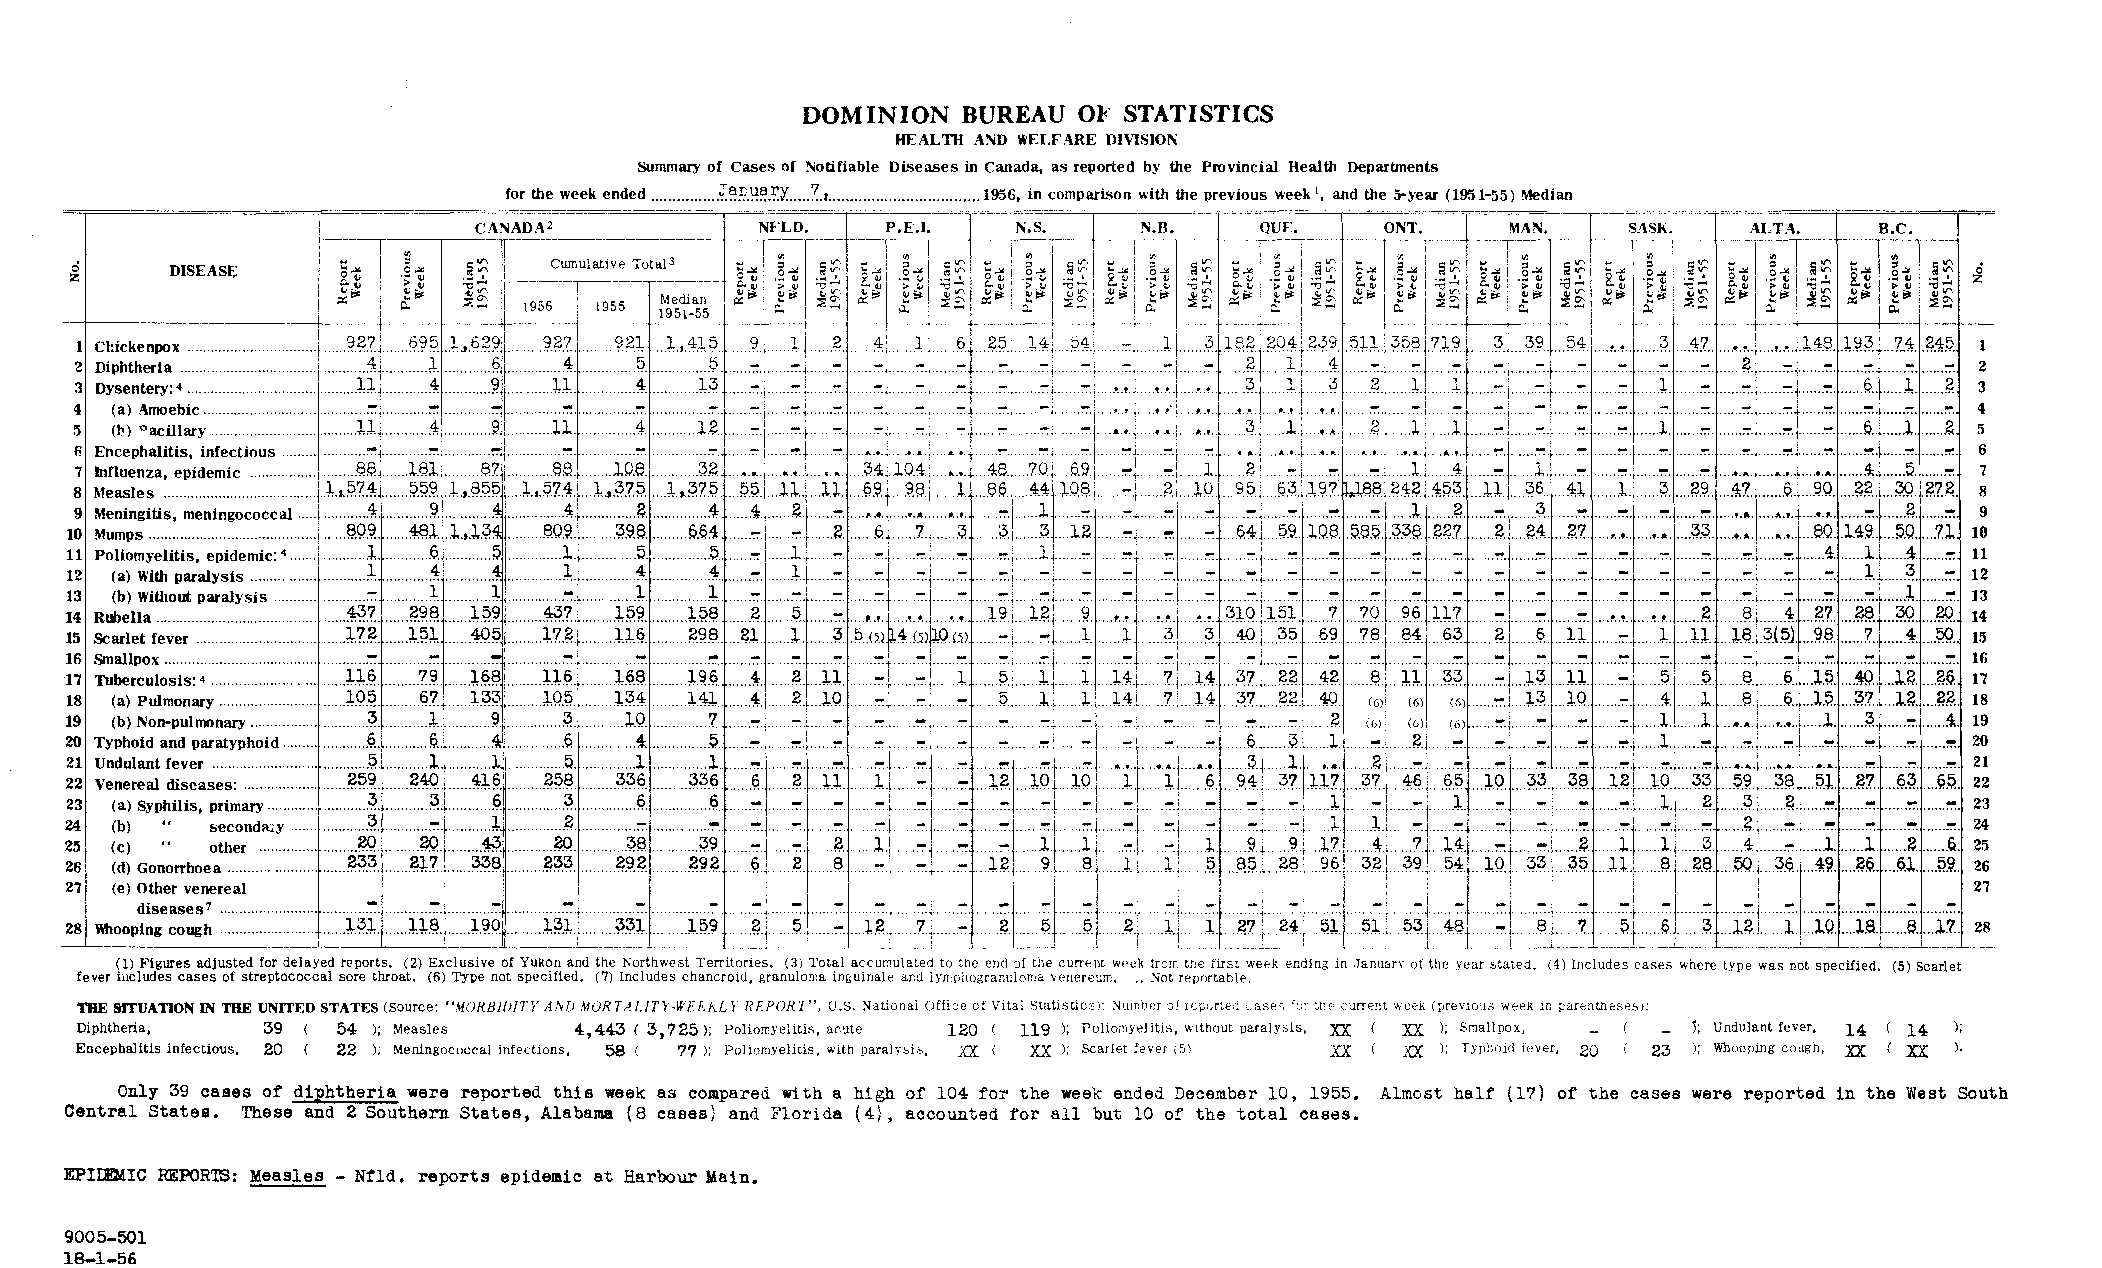
\includegraphics[width=1\linewidth]{figure/cdi_ca_1956_wk_prov_dbs_Part1.pdf}
    \caption{Week 1 table of the Canadian Disease Incidence Dataset. Source: Dominion Bureau of Statistics, 1956; reproduced under Crown copyright's 50-year term (expired at the end of 2006 for a 1956 publication), placing this material in the public domain in Canada.}
    \label{fig:NDD1}
\end{figure}


For a human observer, the table shown in \cref{fig:NDD1} is easily interpretable. However, from the perspective of an OCR engine such as Textract, some problems in the cell contents and structure arise. Below are the common problems seen in the cell structure and content that appear in many historical data documents (and lead to problematic results in \cref{sec:NDD}):

\begin{itemize}
    \item Merged cells: In CANDID, many rows contain merged cells. For instance, the cells listing disease cases for Canada are merged, as are the province names and the header for the cumulative total. As a result, row lengths are inconsistent across the table.
    \item Header values that split the data for the current week, previous week, and median are printed vertically, whereas the rest of the table is printed horizontally.
    \item Where data was missing for the week, the document contains ``..'' as a placeholder.
    \item Where there are no cases, the document contains ``-'' as a placeholder.
    \item There is a lot of information useful for interpreting the data at the bottom of the table. Some cells have parentheses next to them with another number (ranging from 1 to 6) referring to a footnote. These footnotes correspond to how the data was collected, the province/territory it was sampled from, etc. For example, in \cref{fig:NDD1} the value ``5(5)'' is entered for P.E.I. under report week for the row ``Scarlet Fever''. This corresponds to 5 cases of the disease in the province, and the (5) corresponds to the footnote ``Scarlet Fever includes cases of streptococcal sore throat.''
    \item At the bottom of each week's table there is information on data named, ``The situation in the United States''. It is not stored in a tabular format, and was therefore not processed with Textract. This corresponds to Textract's ability to successfully complete the table detection task described in \cref{sec:intro}. However, this is valuable information that a statistician or researcher might need, so it is important to note that the tool we used did not process these data.
\end{itemize}




\section{Statistical Measures} \label{sec:measuresAccuracy}

\subsection{Testing Accuracy of Textract Data Compared to Manually Entered Data}
To assess the accuracy of the CANDID data digitized by Textract, we compared it with the corresponding data digitized by humans in McMaster's Theoretical Biology group, using a myriad of metrics.

We refer to this human-digitized dataset as the \emph{reference transcription} rather than a verified gold standard. It is an independently produced transcription, not a ground truth: like any manual entry process, it is itself subject to error, and we do not assume by definition that it is correct. Where possible, disagreements between the two sources are adjudicated against the original source scan rather than resolved in the reference transcription's favour (see \cref{sec:hardcoding} for an example in which this adjudication instead identified an error in the reference transcription).

\subsubsection{Simple Metrics}
The most straightforward metric, which we call the \emph{exact matched-cell proportion}, is the percentage of cells from the Textract dataset that are exactly the same as the reference transcription. This is not a measure of cells that were correctly digitized, but rather the proportion of cells whose both content and location (row and column index) are equivalent.

This percent equivalent metric was first applied to the raw extracted data, and then again
as the data became progressively more processed through the methods described in \cref{sec:postprocessing}.

\paragraph{Inclusion rule.} We define the evaluated cell set reproducibly, following the implementation in \texttt{postprocessing/combine.ipynb}: each cleaned weekly CSV pair (\texttt{data/textract\_cleaned/1956}, \texttt{data/manual\_cleaned/1956}) is compared position-by-position over the overlapping row and column range, i.e.\ \texttt{min(n\_rows)} by \texttt{min(n\_cols)} between the two files for that week; any rows or columns beyond that overlap (e.g.\ from a length mismatch between the two sources) fall outside this range and are not included in the denominator. Merged-cell handling, header/data-row labelling, footnote-marker treatment, and repeated row indices are resolved upstream during the cleaning stage (\cref{sec:postprocessing}) that produces the \texttt{*\_cleaned} inputs, not by the comparison script itself; the comparison operates on whatever string is present in each cleaned cell. Blank cells and ``\texttt{-}''/``\texttt{..}''/``\texttt{...}'' placeholders are retained and compared as literal strings. A cell counts toward the primary numeric denominator in \cref{tab:pipeline} (n=28,255) if the reference (manual) value consists only of digits with optional thousands separators, regardless of what Textract produced for that cell. A cell counts toward the secondary, numeric-both-sources denominator (n=26,069) only if the Textract value is also numeric by the same rule; cells where either side is empty or a placeholder are excluded from both numeric denominators. The row-shift tolerance (\cref{tab:pipeline}, Stage 2) checks whether a Textract cell matches the reference either in its original column or in the adjacent column one position to the right.

\paragraph{Cells excluded by the overlap restriction.} Because the comparison in \cref{tab:pipeline} scores only the overlapping row/column region of each weekly table pair (the inclusion rule above), it does not score every cell Textract produced. Across the 52 cleaned 1956 tables, the evaluated overlap totals 53{,}872 cells, while the full cleaned Textract bounding grids (\texttt{data/textract\_cleaned/1956}, summed row $\times$ column extent per file) total 61{,}116 cells -- so 7{,}244 Textract cells (11.9\% of the full grid) fall outside the evaluated overlap and are not scored by any of the agreement figures in this paper. These excluded cells are not automatically 7{,}244 additional errors: they can include border/padding rows introduced by the cleaning step, repeated header rows, or other structural artefacts of aligning two independently formatted tables, rather than substantive disease-count cells. We report this count for transparency but have not manually audited the 7{,}244 excluded cells to determine how many are non-trivial content versus padding; this is a scope limitation of the reported accuracy figures (see \cref{sec:limitations}).

\subsubsection{String Differences and Levenshtein Distance} \label{sec:levdist}
To quantify discrepancies between cells with extracted string and their manually entered counterparts, we compute string-level similarity metrics, with a primary focus on Levenshtein distance \cite{Levenshtein1965BinaryCC}. Levenshtein distance measures the minimum number of single-character edit operations -- insertions, deletions, or substitutions -- required to transform one string into another; a distance of zero indicates an exact match, while larger values reflect increasing divergence. The standard dynamic-programming recurrence for computing it is given in \hyperref[sec:supp]{Supplementary Material} (S4).

The dynamic-programming formulation above follows the general string-to-string correction framework of Wagner and Fischer \cite{wagner1974string}. In practice, Levenshtein distance is often normalized by string length to enable fair comparison across tokens of different sizes. This is particularly important when evaluating OCR output, where short strings (e.g., years or counts) are disproportionately sensitive to single-character errors.


\subsection{Epidemiologically Significant Statistics Derived from Textract Data}

\subsubsection{Row and Column Sums}
Aggregate counts obtained by summing across diseases or locations are often needed.  If these sums were provided in the original documents, then they also provide a valuable opportunity for consistency checks in the data entry. Thus, it is extremely useful to sum values across a row or down a column and confirm that the result matches the reported total at the end of that row or column. If the sums agree, it provides an immediate check that entries were not missed, duplicated, or mistyped. While it is technically possible for errors in both the extracted sums and incidence values to cancel out and still agree, this is very unlikely. Discrepancies immediately flag rows or columns that require closer review, allowing errors to be identified and corrected early before downstream analysis.

\subsubsection{Cross-Correlation Between Diseases}
Computing cross-correlation between two disease time series involves measuring how strongly their observed patterns move together over time, and whether changes in one disease tend to occur before, after, or at the same time as changes in the other. Instead of determining whether two diseases are correlated in a broad sense, cross-correlation
examines their relationship across different time shifts. For example, whether peaks in Measles are followed by peaks in Chickenpox one or two weeks later. Mathematically, it compares the standardized values of one time series with shifted versions of the other, producing a correlation value for each lag.

Ordinary correlation measures the linear association between two random variables $X$ and $Y$. 
It is defined as the normalized covariance.
This quantity lies in $[-1,1]$ and measures the strength and direction of linear dependence.

For time series $\{x_t\}$ and $\{y_t\}$, ordinary correlation corresponds to comparing values at the same time index:
\[
\rho_{xy}(0) = 
\frac{\mathrm{Cov}(x_t, y_t)}{\sigma_x \, \sigma_y}.
\]

Cross-correlation extends this idea by introducing a time shift, which is called the lag. 
The cross-covariance at lag $k$ is
\[
\gamma_{xy}(k) = \mathrm{Cov}(x_t, y_{t-k}),
\]
and the cross-correlation function (CCF) is
\[
\rho_{xy}(k) = 
\frac{\gamma_{xy}(k)}{\sigma_x \, \sigma_y}.
\]

Thus, $\rho_{xy}(k)$ is the correlation between $x_t$ and a shifted version of $y_t$. 
By varying $k$, cross-correlation measures linear dependence across different time offsets.

\paragraph{Interpretation:}
\begin{itemize}
    \item $k = 0$: simultaneous association.
    \item $k > 0$: $x$ leads $y$ by $k$ time units.
    \item $k < 0$: $y$ leads $x$ by $|k|$ time units.
\end{itemize}



We will compute the cross correlation function, CCF, $\rho_{xy}(k)$ with $x$ and $y$, referring to two different diseases that were both reported during our time period. Our objective is to compute the CCF using the manually curated data, and then compute the same CCF using the automatically extracted data. This produces two cross-correlation sequences corresponding to the manual and extracted datasets, respectively. If the two CCFs are sufficiently similar, we will conclude that the automatic data extraction is sufficiently accurate to make epidemiologically meaningful inferences.


To assess similarity, we compare these functions across all lags $k$. This can be done by examining differences in (i) the lag at which the maximum correlation occurs, (ii) the magnitude of peak correlations, and (iii) the overall shape of the CCF curves. Quantitatively, one may compute the difference 


\[
\Delta(k) = \rho_{xy}^{\mathrm{T}}(k) - \rho_{xy}^{\mathrm{M}}(k),
\]
where superscripts M and T refer to manual and Textract data, respectively.  If the two CCFs are similar in magnitude, peak location, and overall structure, this suggests that the extracted data preserves the dependence structure present in the manual dataset.


\subsubsection{Other Time Series Statistics}

Another verification tactic is to filter the data by disease---or more generally, by category or type---and examine each subset independently. Analyzing grouped data makes it easier to spot values that are inconsistent with the typical range for that specific group. Outliers can then be identified by visual inspection of scatterplots, boxplots, interquartile range, or standard deviation-based cutoffs.

Using more than one approach reduces the risk of missing meaningful anomalies or over-flagging valid but extreme observations, and helps distinguish true data entry errors from legitimate but rare values.

The test statistics of greatest interest are those that an epidemiologist would be naturally interested in calculating. In a time series of disease incidence, the \emph{peak height} is simply the largest observed value (the maximum number of cases), and the \emph{peak time} is the time index or date at which this maximum occurs. For a time series of a given disease, knowing the peak height and the time at which it occurs is important as it helps predict the intensity of an outbreak.

\paragraph{Peak-detection rule (\crefrange{table:measles_growthrate_results}{tab:growthrateschickenpox}).} Because a raw weekly maximum is sensitive to isolated OCR spikes and single-week noise, peaks are located from a locally smoothed series rather than the raw weekly values: within each fitting window, we fit a local quadratic regression (LOESS, span $0.4$, degree 2) to weekly cases against week index, and report the week and fitted value at which this smoothed curve is maximized. Ties in the smoothed maximum resolve to the earliest week in the window. Weeks with a missing time index or missing case count are dropped prior to smoothing rather than imputed; a window is not fit if fewer than 5 non-missing weeks remain. We separately checked whether any reported peak week (Measles: weeks 64 and 126; Chickenpox: weeks 64, 112, and 114) coincides with a week flagged by the row-sum validation of \cref{sec:hardcoding}: none can be checked, because that validation covers only the 52 weeks of 1956, while every reported peak here falls in 1957 or 1958. This is itself a limitation of the current validation coverage, not evidence that the reported peaks are error-free.

In the context of analyzing the quality of our extracted data, testing the growth rate is important as it is one of the preliminary statistics that researchers want to know about an epidemic. Estimating the initial growth rate of a disease time series quantifies how quickly the number of cases increases during the early phase of an outbreak. The growth rate provides a concise measure of epidemic speed and can be used to compare outbreaks across locations or time periods. The early phase of an outbreak is typically well-approximated by exponential growth, where the expected number of cases increases proportionally to the current number of cases. The initial exponential growth rate, which we denote $r$ throughout this paper, is particularly important as it yields the epidemic doubling time ($\frac{\ln{2}}{r}$); in principle it can also be used to derive quantities such as the basic reproduction number $\mathcal{R}_0$ \cite{WallLips07}, though we do not compute $\mathcal{R}_0$ in this paper and mention it only as context for why $r$ is a quantity of independent epidemiological interest, not only an intermediate step toward the doubling time.

Methods for estimating the initial exponential growth rate \cite{Ma2014,JaganRpkg} typically take advantage of the fact that if incidence is growing exponentially then cumulative incidence also grows exponentially. Since datasets are often observed at substantial intervals (e.g., weekly), designing methods that use ``interval incidence'' (the difference between cumulative incidence at observation times) is more robust. We can also use the growth rate to calculate the doubling time, which is a statistic that is more easily interpreted numerically.
The exponential growth rate \(r\) is related to the doubling time $T_{\mathrm{d}}$ by
\[
T_{\mathrm{d}} = \frac{\ln 2}{r}
\]

\paragraph{Model specification (\crefrange{table:measles_growthrate_results}{tab:growthrateschickenpox}, \crefrange{fig:growthratesm}{fig:growthrateschickenpox}).} Growth rates and doubling times for Measles and Chickenpox were estimated with \texttt{epigrowthfit} 0.15.5 \cite{JaganRpkg} in R 4.5.1, using \texttt{egf\_model(curve = "logistic")} with all other model arguments left at their package defaults (negative-binomial dispersion, no day-of-week effect -- not applicable, since our data are weekly rather than daily -- and no excess-cases term). Every top-level model parameter, including $\log(r)$, used the default intercept-only formula, so a single growth rate $r$ was estimated jointly from both fitting windows for a given disease and data source, rather than a separate rate per window; \cref{sec:NDD} reports what this implies for the two-window presentation in \crefrange{fig:growthratesm}{fig:growthrateschickenpox}. Confidence intervals are Wald intervals computed on the $\log(r)$ scale via \texttt{confint.egf()} and back-transformed. The two fitting windows (week 35--64 and week 95--126, bracketing the two annual epidemic waves visible in the incidence curves) were chosen by visual inspection of the manually entered time series and then applied unchanged to the corresponding Textract series for the same disease; windows were not re-chosen from the Textract data itself. Weeks with a missing time index or case count inside a window are dropped prior to fitting, matching the treatment used for peak detection above.

\section{Analyzing the results from the Canadian Disease Incidence Dataset} \label{sec:NDD}
The following section explores the accuracy of table extraction on a particular dataset, namely the Canadian Disease Incidence Dataset (CANDID). 


\subsection{Comparison to Manually Entered Data}
\subsubsection{Simple Metrics}\label{sec:simple}
The cell-agreement analysis in this section covers the 1956 CANDID tables only, not the full 1956--1958 (156-table) dataset described in \cref{sec:NDDdetails}. It was computed with the evaluation script in \texttt{postprocessing/combine.ipynb}, run over the 52 weekly tables for 1956 (53{,}872 evaluated cells in total; 26{,}069 of these hold numeric values on both the Textract and reference sides). When comparing values cell by cell, the percentage of cells between the raw Textract data and the manually entered reference transcription that were equivalent (both content and position, i.e.\ strict string equality; see \cref{sec:measuresAccuracy}) was 74.0\% across all evaluated cells, or 71.9\% among the 28{,}255 cells numeric in the manual reference (77.9\% if instead restricted to the 26{,}069 cells numeric on both sides). Applying a sequence of processing stages to the Textract output increased content-only agreement (tolerant of comma/whitespace formatting and of a value being shifted into an adjacent column) to 88.5\% across all cells, and to 92.9\% among cells numeric in the manual reference -- the primary numeric-accuracy figure used in this paper, since it does not exclude cells where Textract failed to extract any number at all (a secondary figure of 95.6\% obtains under the numeric-on-both-sides denominator). \Cref{tab:pipeline} summarizes each stage, its resulting agreement under all three denominators, and, critically, whether the underlying rule was fixed independently of this dataset (\emph{a priori}), developed by inspecting the reference transcription, or applied as a manual, post-hoc correction. This distinction matters because rules developed by inspecting the reference data are not validated against unseen material (see the leakage discussion in \cref{sec:limitations}).

\begin{table}[h]
\centering
\footnotesize
\begin{tabularx}{\textwidth}{c X >{\centering\arraybackslash}p{2.1cm} >{\centering\arraybackslash}p{2.1cm} >{\centering\arraybackslash}p{2.1cm} X}
\toprule
Stage & Operation & All cells (n=53{,}872) & Numeric, manual ref.\ (n=28{,}255) & Numeric, both sources (n=26{,}069) & Rule provenance \\
\midrule
0 & Raw Textract output (strict equality) & 74.0\% & 71.9\% & 77.9\% & --- \\
1 & + Comma/whitespace normalization & 76.8\% & 77.3\% & 83.8\% & generic, a priori \\
2 & + Row-shift tolerance (adjacent column) & 88.5\% & 92.9\% & 95.6\% & developed against reference data \\
3 & Manual correction following inspection (Meningitis, Mumps) & not quantified & not quantified & not quantified & manual, post-hoc \\
\bottomrule
\end{tabularx}
\caption{Pipeline stages applied to the raw Textract output for the 1956 CANDID tables, and the resulting cell-agreement percentage at each stage under three denominators, as computed by \texttt{postprocessing/combine.ipynb} and exported to \texttt{data/analysis\_intermediates/accuracy\_summary.csv}. Stage 2 reports content-only agreement (a match either in place or shifted one column over); it is not a strict content-and-position metric. The primary numeric-accuracy figure used elsewhere in this paper is the ``Numeric, manual reference'' column (n=28{,}255: every cell where the manual transcription holds a numeric value, regardless of what Textract read there), since it does not silently exclude cells where Textract failed to extract a number at all. The ``Numeric, both sources'' column (n=26{,}069) is reported as a secondary figure for comparability with denominators used elsewhere in the OCR-evaluation literature.}
\label{tab:pipeline}
\end{table}
\subsubsection{String Differences}
Using Python's NLTK library and its Levenshtein distance function, it is relatively straightforward to find the Levenshtein distance between two strings. The goal is to find the distribution of edit distances among mismatched entries, from cells differing by a single character to cells with little resemblance to the reference value. It is illustrative to find the average distance from entries where an actual error occurs. Recall from \cref{sec:simple} that content-only agreement (tolerant of comma/whitespace formatting and of a value being shifted into an adjacent column) is 88.5\% across all evaluated cells; this is distinct from the strict content-and-position agreement of 74.0\%, in which a cell's content may be correct but extracted to the wrong location within a table. In the analysis below, ``mismatched'' cells are those failing even the content-only criterion (\texttt{Any\_Equality = False} in the evaluation script), i.e.\ the residual disagreements not resolved by any of the processing stages in \cref{tab:pipeline}. The average Levenshtein distance among these mismatched cells is approximately 1.84. Separately, the modal distance is 2 (51.7\% of mismatched cells), with 1 the next most common (38.1\%). \cref{fig:Ldist} shows the proportion of cell contents per Levenshtein distance.

\begin{figure}
    \centering
    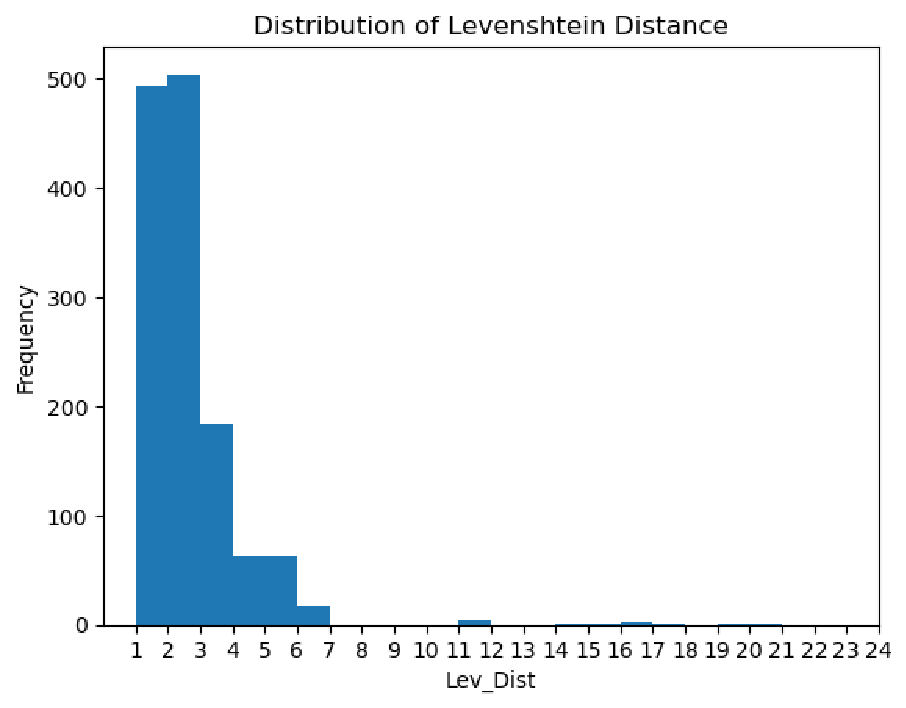
\includegraphics[width=0.7\linewidth]{figure/Lev_dist.pdf}
    \caption{
The frequencies of Levenshtein Distances (defined in \cref{sec:levdist}) between manual and Textract cell values in the CANDID. The majority of distances measured are 1 or 2 differences in characters between the two strings.}
    \label{fig:Ldist}
\end{figure}

We see the most common Levenshtein distances are as expected, namely distances of 1 or 2. This aligns with results from \cref{sec:simple}, where most cell contents differ by a single digit or special character. Of the tables for 1956, 6{,}177 of 53{,}872 evaluated cells (11.5\%) were cells that we considered to have true extraction errors (i.e. mistakes that were not resolved through post-processing); of these, 38.1\% have a Levenshtein distance of 1 and 51.7\% have a Levenshtein distance of 2.

The distance value then drops off steeply after a distance of 2, with a thin tail extending out to a maximum of 25. It is likely the OCR engine confuses a blurry part of a number, or that the structure of the table or quality of scan precludes accurate extraction of one or two digits.

The percentage of each Levenshtein distance in cells with errors from the tables for 1956 is seen in \cref{tab:lev_dist}.

\begin{table}[h]
\centering
\begin{tabular}{ccc}
\hline
\textbf{Levenshtein Distance} & \textbf{Count} & \textbf{Percentage} \\
\hline
1  & 2356 & 38.14\% \\
2  & 3194 & 51.71\% \\
3  & 314  & 5.08\%  \\
4  & 98   & 1.59\%  \\
5  & 114  & 1.85\%  \\
6  & 84   & 1.36\%  \\
8  & 3    & 0.05\%  \\
9  & 2    & 0.03\%  \\
11 & 7    & 0.11\%  \\
14 & 4    & 0.06\%  \\
25 & 1    & 0.02\%  \\
\hline
\end{tabular}
\caption{Distribution of Levenshtein distances between extracted and reference values, computed by \texttt{postprocessing/combine.ipynb} over the 1956 CANDID tables. Counts sum to 6{,}177 cells with true extraction errors, out of 53{,}872 evaluated cells.}
\label{tab:lev_dist}
\end{table}

There are outliers in the trend seen at Levenshtein distances of 8, 9, 11, 14, and 25. These errors are almost certainly specific to this dataset and processes. For example, the single distance-25 outlier corresponds to a cell where Textract returned a run of placeholder dots (\texttt{.........................}) instead of a value, compared against the reference value \emph{68}: the entire reference string had to be inserted character-by-character, producing a large Levenshtein distance. The specific Levenshtein distances, and where they are located, would depend on the structure and content of the table in question. We can expect that longer strings, or cells where Textract fails to extract any numeric content at all, would contribute to a larger Levenshtein distance.

For Levenshtein distances greater than 6, the errors we inspected occur in the disease-name column (column index 0) of the affected tables, where Textract extracted a word or word-fragment (e.g.\ ``\,meningococcal'', ``\,infectious'', ``\,epidemic'', ``\,primary'') into a cell the reference transcription records as a plain numeric value or placeholder. This pattern is consistent with row misalignment: a multi-word or multi-row disease-name label bleeding into the row Textract assigned to the adjacent numeric entry.

Of course, Levenshtein distances of large magnitudes help us in the sense that, following a manual inspection of the extracted data, it would be clear to a human that an error has occurred. In addition, distances of this magnitude were concentrated in disease-name strings and row-alignment failures rather than in numeric values.

We also looked at the relative Levenshtein distance, i.e., the Levenshtein distance proportional to the length of the reference string. This allows us to visualize the errors caused by Textract in a way that accounts for the length of the string
 (see \cref{fig:LdistNormal}). As longer strings have a higher potential Levenshtein distance, normalizing by their lengths aids in determining the proportion of mistakes.
\begin{figure}[H]
    \centering
    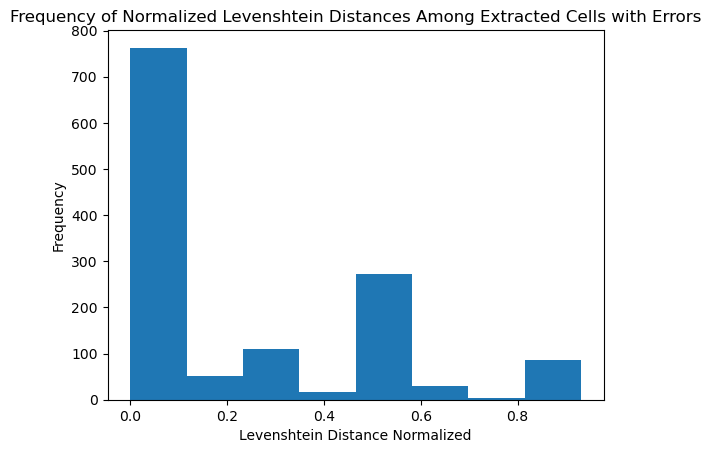
\includegraphics[width=0.7\linewidth]{figure/normalized_L.png}
    \caption{Levenshtein Distance (as defined in \cref{sec:levdist}) normalized by the length of the string of the manually entered cell value.}
    \label{fig:LdistNormal}
\end{figure}
In cells with errors, we see that the most common values of normalized Levenshtein distance is 0.1. 
The other spikes in the graph, around 0.5 and greater than 0.9 can be attributed to shifted cells. For example, when Textract inputs the name of a disease in a cell location that is expected to be a disease count, the character counts between the Textract and manual cell values will vary greatly.
\clearpage

\subsubsection{Detecting Minor Errors with Row Sums}
To mitigate errors arising from row misalignment during extraction, rows corresponding to the same disease were first grouped from each table. Because similar shifting occurs for the same disease in each table, grouping rows by disease prior to checking row sums makes it possible to enforce consistent indexing and ensure that computed quantities are evaluated over the correct set of entries. The structure of the data used for this computation is illustrated in \cref{fig:sumrows}. The total incidence value for the week is in a column titled ``report week'' under ``Canada'' and the contributing cell values similarly appear every third column for each province and territory. 

\begin{figure}[H]
    \centering
    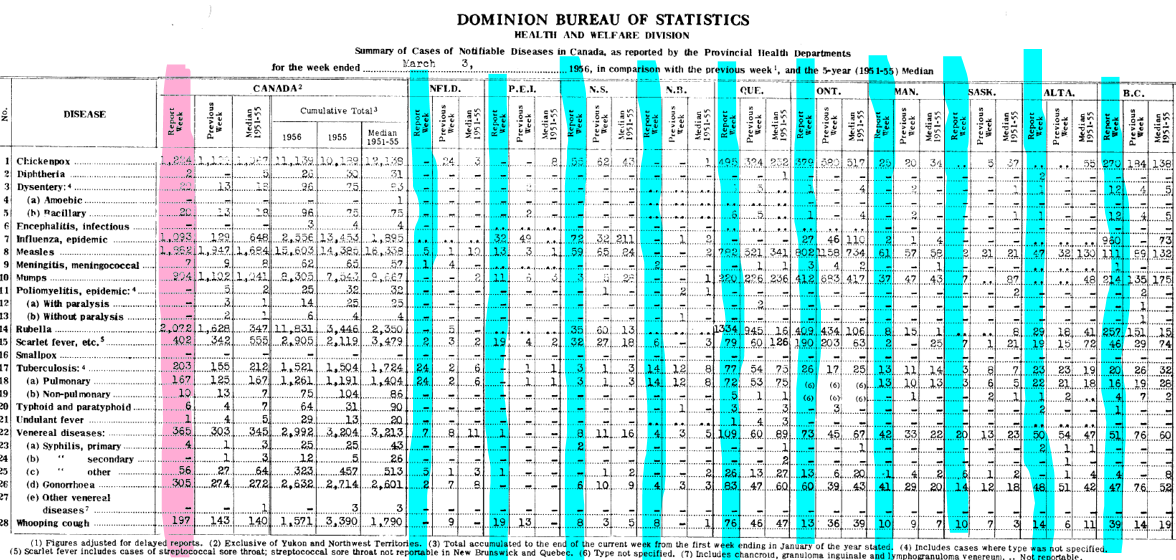
\includegraphics[width=0.75\linewidth]{figure/computing-sums.png}
    \caption{Rows contributing to the computed sums are in blue, and the expected sums are in pink, of the tables in CANDID \cref{sec:NDDdetails}. In the original PDF table, we expect that across a row, the sum of each value in the blue columns equals the total in pink.}
    \label{fig:sumrows}
\end{figure}

By disease, we plot the difference between the expected sums, as extracted by Textract, and the actual sum calculated by looping over the row contents. Below are the values calculated for Chickenpox (see \cref{fig:chickenpoxsum}).

\begin{figure}
    \centering
    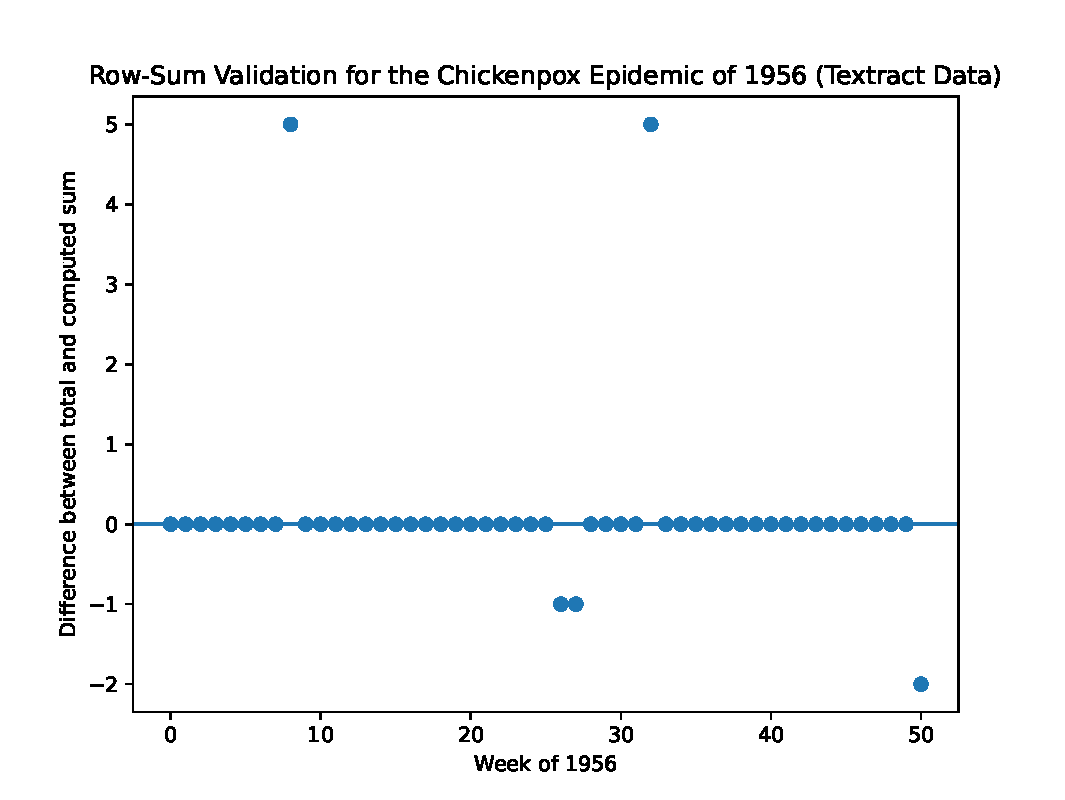
\includegraphics[width=0.7\linewidth]{figure/Chickenpox.pdf}
    \caption{Differences in expected versus calculated row sums for Chickenpox in CANDID (\cref{sec:NDDdetails}) to verify accuracy of cell values (method described in \cref{sec:measuresAccuracy}).}
    \label{fig:chickenpoxsum}
\end{figure}

Most rows exhibit zero difference, indicating agreement between extracted totals and recomputed values. Nonzero deviations indicate inconsistencies that can be traced to numerical errors in individual cells. 



For example, the first outlier in \cref{fig:chickenpoxsum} corresponds to Week 9 in the dataset. From inspecting the scan of the table, we find the true total is \textit{1224}, computed from the non-empty contributing values:

\[55,495,379,25,270\]


In the extracted version of the dataset, Textract correctly extracts the total to be \textit{1224} from the table, but differs from the reference values on the actual contributing incidents values:

\[50,495,379,25,270\]

Our algorithm found these values and calculated the sum, which is $1,219$. So the difference between the expected sum and the calculated sum is 5, as seen in \cref{fig:chickenpoxsum}. A direct comparison shows that the value 55 was misread as 50. In this way, relatively minor numerical discrepancies can be found and corrected.


Some discrepancies are more subtle. For instance, the first outlier in \cref{fig:measlessum} corresponds to Week 9. The recomputed total from the extracted contributing values is:

\[5,13,59,782,802,61,2,47,111\].


Textract reports a total of \textit{1852}, while the sum of the contributing values equals \textit{1882}. This gives the difference of $-30$ in \cref{fig:measlessum} at week 9. This inconsistency indicates that there exists an error from either the contributing cells or the extraction of the row total, or both. When we compared these values to the scanned document, we found that the reference transcription records the row total as \textit{1862} (see \cref{fig:1882}), which differs from Textract's reported total of \textit{1852} by only \textit{10} -- but a 10-count discrepancy between the two transcriptions does not explain the original 30-count gap between Textract's total and the sum of the contributing values. A further gap of \textit{20} (\textit{1882} minus \textit{1862}) separates the reference transcription's total from the sum of the contributing values.

Upon closer inspection of the source image, the correct value in the scan of the total is \textit{1882} (exactly the sum of the contributing values). This highlights an error in the reference transcription, not the Textract extraction, coming from the ambiguity of the original scan. This is a substantive result in its own right: row-sum validation detected an error in the reference transcription rather than in the Textract output, demonstrating that internal consistency checks can adjudicate between the two sources rather than merely score the extraction tool against an assumed-correct reference (see also the Discussion in \cref{sec:limitations}).

\begin{figure}[H]
    \centering
    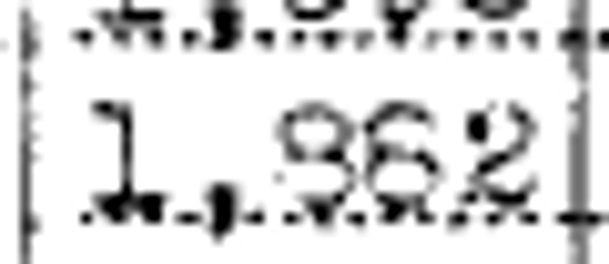
\includegraphics[width=0.10\linewidth]{figure/1882.png}
    \caption{Total Measles instances in Week 9 of CANDID. This is hard to interpret for both OCR and humans.}
    \label{fig:1882}
\end{figure}

These examples illustrate an important advantage of the row-sum validation approach: it detects small inconsistencies in numerical cell contents, and this approach can be adapted for the detection of OCR errors. By comparing independently computed totals with reported values, the method provides a mechanism for flagging anomalies in the dataset.
\begin{figure}
    \centering
    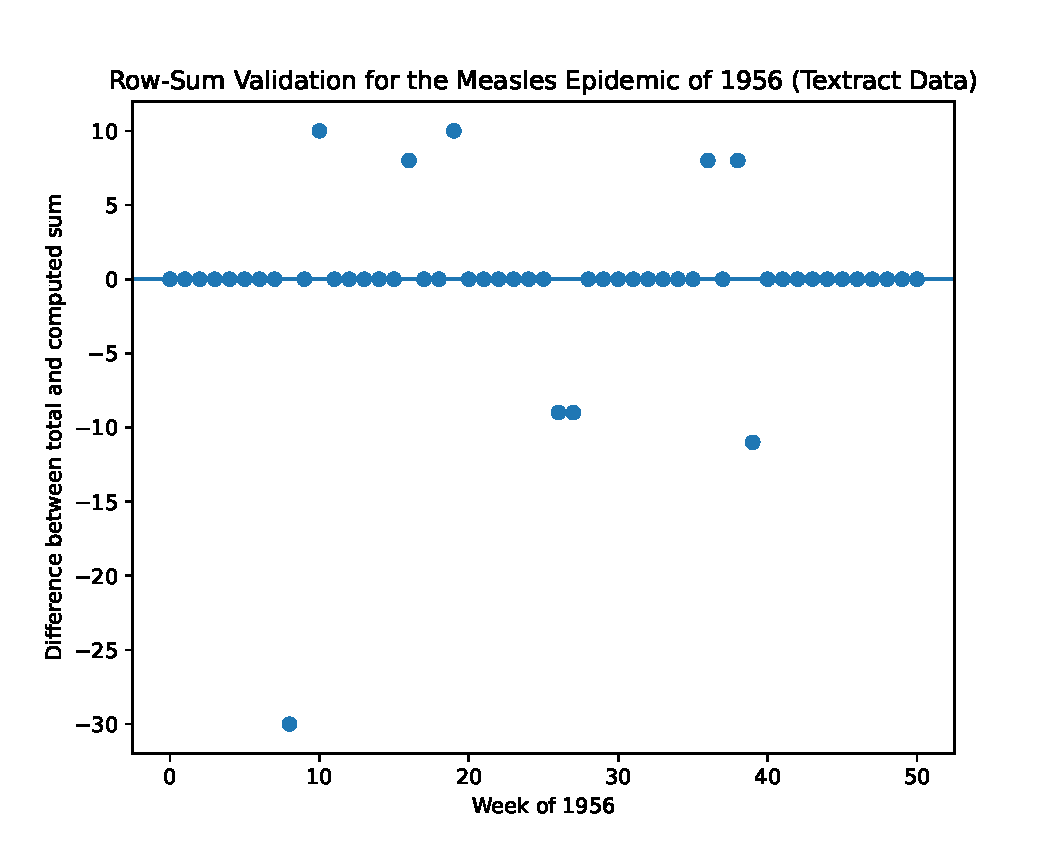
\includegraphics[width=0.7\linewidth]{figure/Measles.pdf}
    \caption{Differences in expected versus calculated row sums for Measles in CANDID (\cref{sec:NDDdetails}) to verify accuracy of cell values (method described in \cref{sec:measuresAccuracy}).}
    \label{fig:measlessum}
\end{figure}

\clearpage
\subsection{Comparing Important Statistics}

\subsubsection{Cross-Correlation Between Diseases}

Unless otherwise stated, the Textract series used in this subsection are the processed data described in \cref{tab:pipeline} (Stage 2), without manual correction. The cross-correlation analysis presented first focuses on the relationship between Chickenpox and Measles epidemics. This involved extracting the relevant time series from both the manually curated dataset and the Textract extraction, followed by post-processing to align formats, handle missing values, and ensure consistent indexing across both sources (see \cref{sec:postprocessing}).

To provide an initial qualitative assessment of the relationship between these diseases, and to evaluate the accuracy of the extracted data, we plot the time-series of both datasets \cref{fig:comparisonIncidents}. Visually, the two series are highly similar, indicating that the extraction process preserves the overall timing structure of the data. 

This observation is consistent with the quantitative results reported in \cref{sec:simple}, where it was established that content-only agreement (tolerant of formatting and of a value shifted into an adjacent column) is 92.9\% for cells numeric in the manual reference (95.6\% under the numeric-on-both-sides denominator), with most remaining errors involving only small numerical deviations. As a result, the dominant trends, seasonal patterns, and relative magnitudes of the two diseases are largely unaffected by extraction noise. The remaining disagreements do change the graphs slightly. At around week 60, there is a sharp decrease in Chickenpox, and around week 145, there is some Measles data missing. This is also unsurprising to see in the Textract data, which contains errors that are systematic and sharp; for example, the Scarlet Fever comma-induced shift described in \cref{sec:hardcoding} propagates through all affected rows rather than occurring at random.





\begin{figure}[h!]
    \centering
    
    \begin{subfigure}[b]{0.48\textwidth}
        \centering
        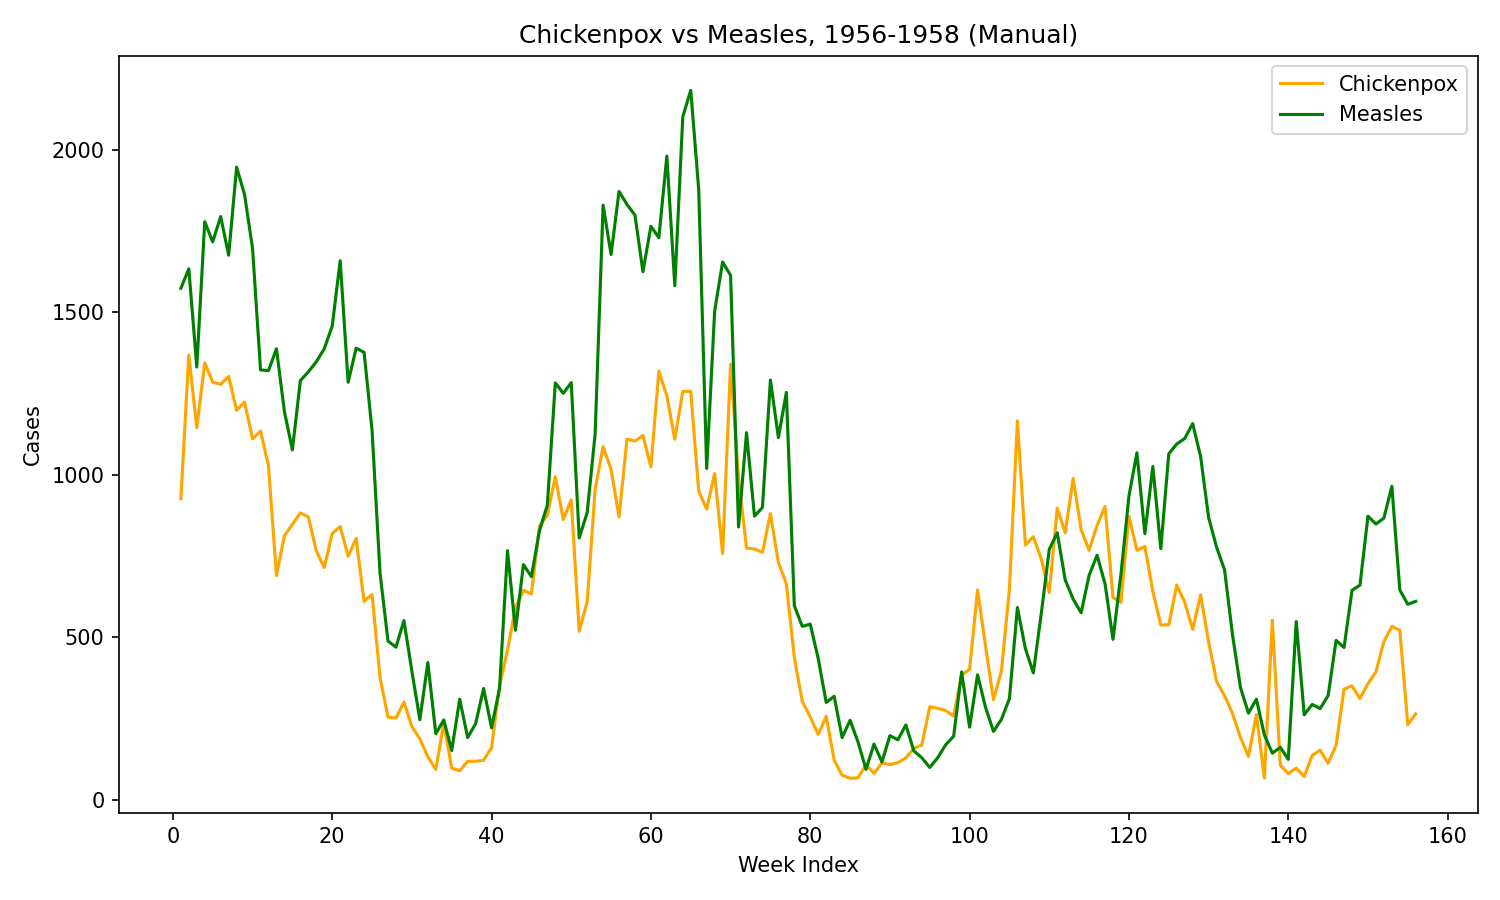
\includegraphics[width=\textwidth]{figure/MeaslesvsChickenpoxmanualdata.png}
    \end{subfigure}
    \hfill
    \begin{subfigure}[b]{0.48\textwidth}
        \centering
        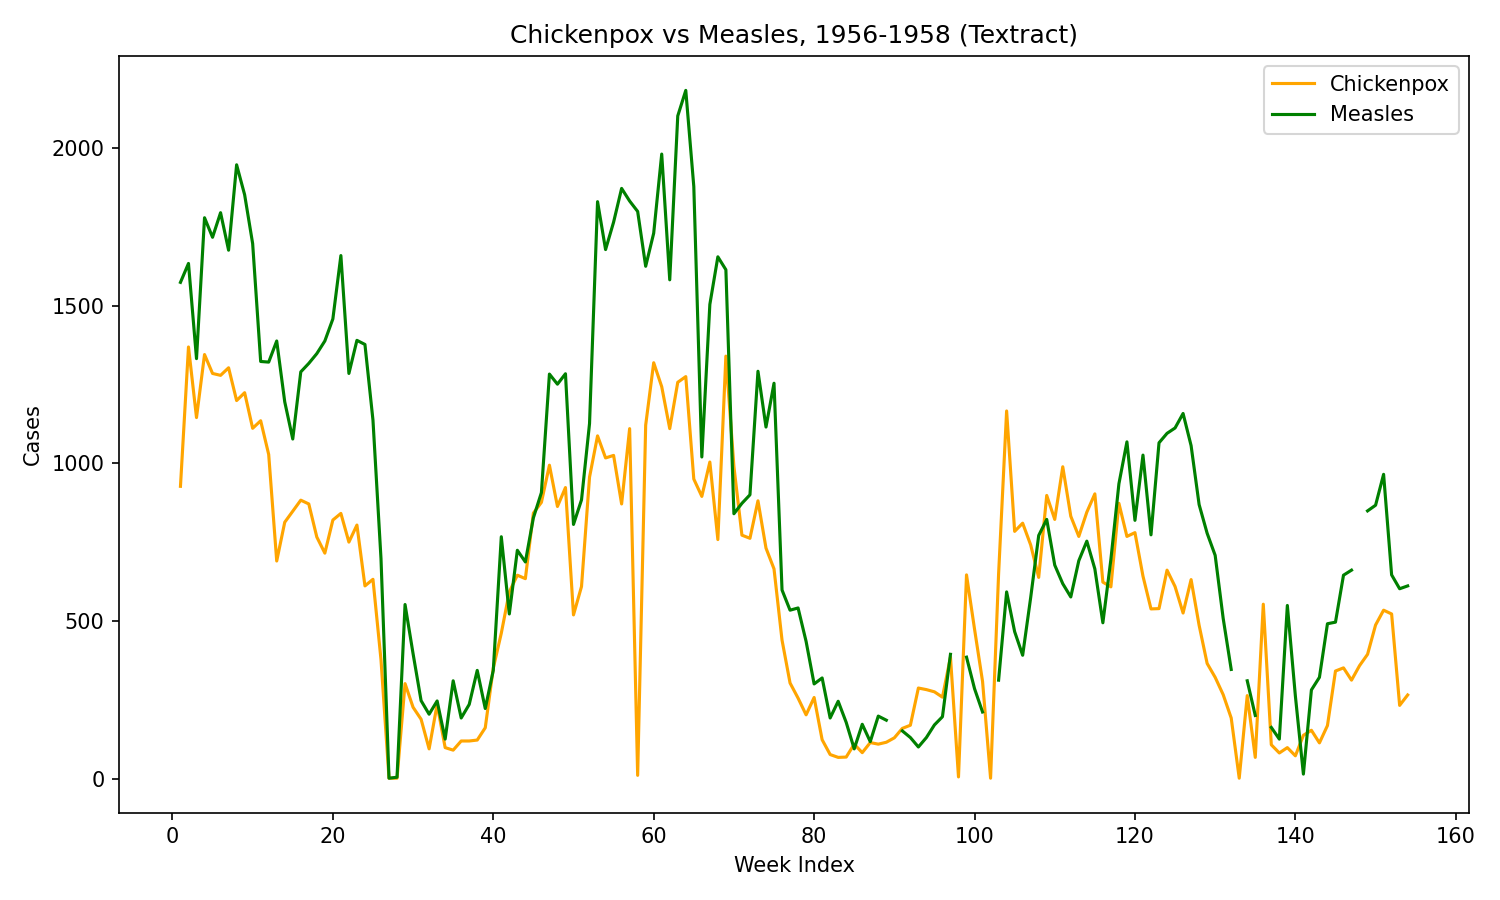
\includegraphics[width=\textwidth]{figure/MeaslesvsChickenpoxtextract.png}
    \end{subfigure}
    
    \caption{Comparison of manual versus Textract disease incidence for Chickenpox and Measles. Data version: Textract series processed through the pipeline in \cref{tab:pipeline} (Stage 2), without manual correction.}
    \label{fig:comparisonIncidents}
\end{figure}

The two series rise and fall in roughly the same seasonal pattern, with major peaks and troughs occurring at approximately the same times. Thus, from the incidence curves alone, we would expect a fairly strong positive cross-correlation at lag 0. The cross-correlation function would likely show its maximum at or very near lag 0, with a value that is moderately high after standardization.

For our purposes, it is critical to examine the difference between the cross-correlation computed between the manual and Textract data. The graphs for both computations are shown in \cref{fig:comparisonCrossCorrelation}; the quantified comparison follows below (\cref{tab:ccf_summary}).

\begin{figure}[h!]
    \centering
    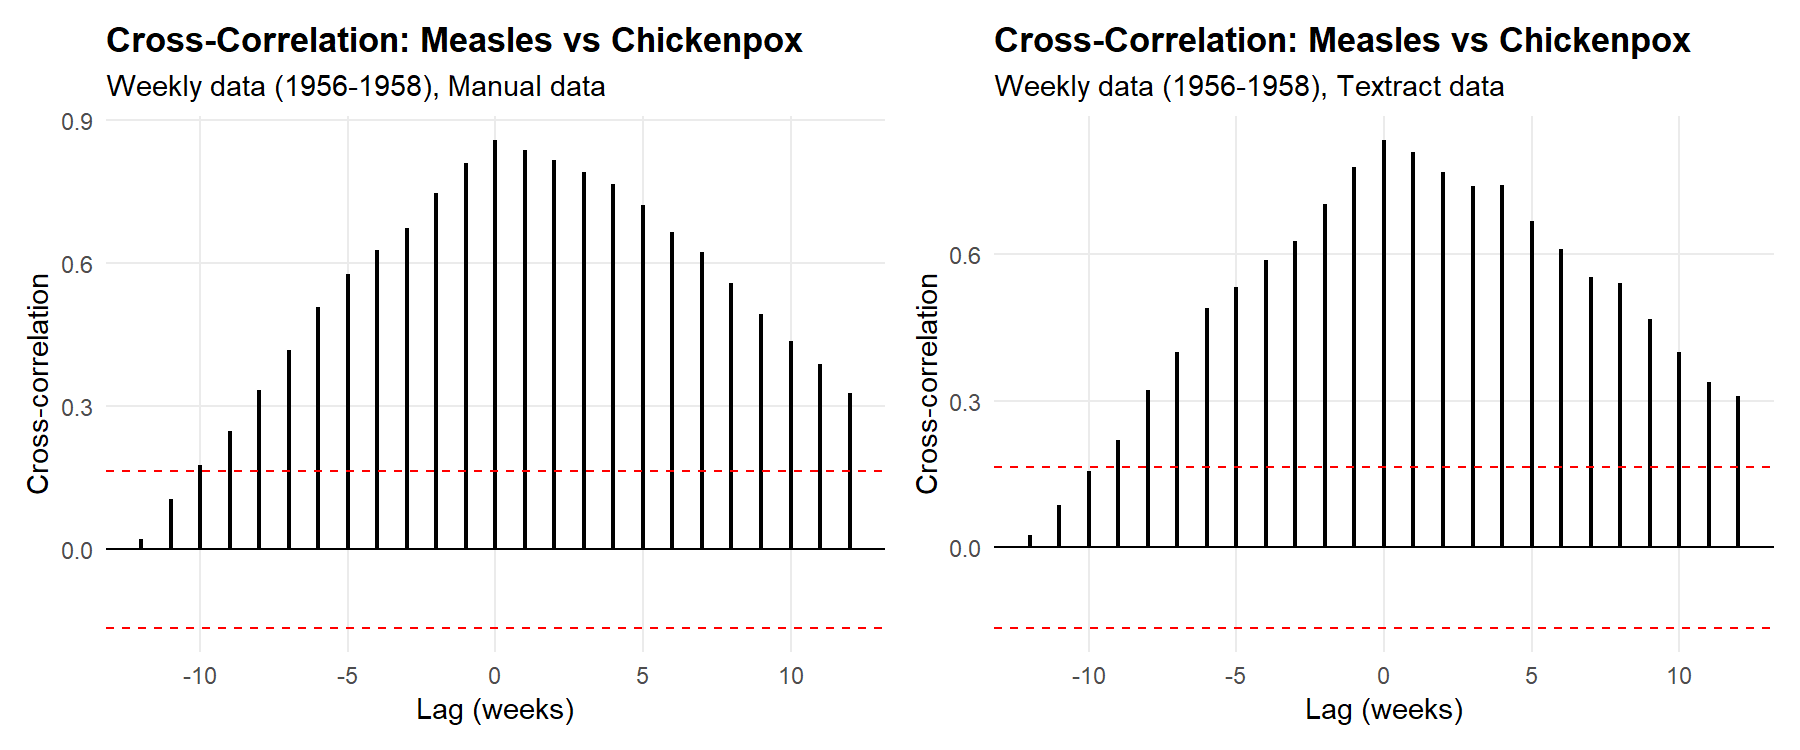
\includegraphics[width=\linewidth]{figure/fig11_measles_chickenpox_ccf.png}
    \caption{Comparison of manual versus Textract disease cross-correlation for Chickenpox and Measles. This is described in \cref{sec:measuresAccuracy}. Data version: processed Textract data (\cref{tab:pipeline}, Stage 2), without manual correction. Regenerated from the corrected common-calendar-week CCF calculation (\texttt{analysis/cross\_correlation.R}); see \cref{tab:ccf_summary}.}
    \label{fig:comparisonCrossCorrelation}
\end{figure}

To gain a sense of how similar the cross-correlations are, we computed a set of summary statistics across all lags (\cref{tab:ccf_summary}; per-lag values are in \hyperref[sec:supp]{Supplementary Material}, Table S1). We report absolute and root-mean-square differences rather than a relative difference at each lag, because a relative difference is uninformative wherever the manual correlation is itself near zero, as the next comparison illustrates.

Both datasets peak at lag 0 (\cref{tab:ccf_summary}), so the change in peak lag is 0 and the change in peak correlation is small ($-0.0255$). Across all 25 lags, the largest absolute discrepancy between the two series is $0.0699$ (at lag 7) and the root-mean-square difference is $0.0376$. In this disease-pair comparison, the lag with the highest cross-correlation was unchanged after processing. Because cross-correlation is a measure of time relationships rather than exact magnitudes, the estimated timing structure of this pairwise comparison was similar between the two sources.

We repeat this process with the time series for Measles and Meningitis (incidence curves in \cref{fig:comparisonIncidentsMM}, cross-correlation in \cref{fig:comparisonCrossCorrelation2}), and compare the values using the same summary statistics (\cref{tab:ccf_summary}; per-lag values are in \hyperref[sec:supp]{Supplementary Material}, Table S2). Unlike the Measles/Chickenpox comparison above, the Meningitis series used here has been manually corrected: additional post-processing was applied to remove visible outliers, as described in \cref{sec:hardcoding}.


\begin{figure}[H]
    \centering
    
    \begin{subfigure}[b]{0.48\textwidth}
        \centering
        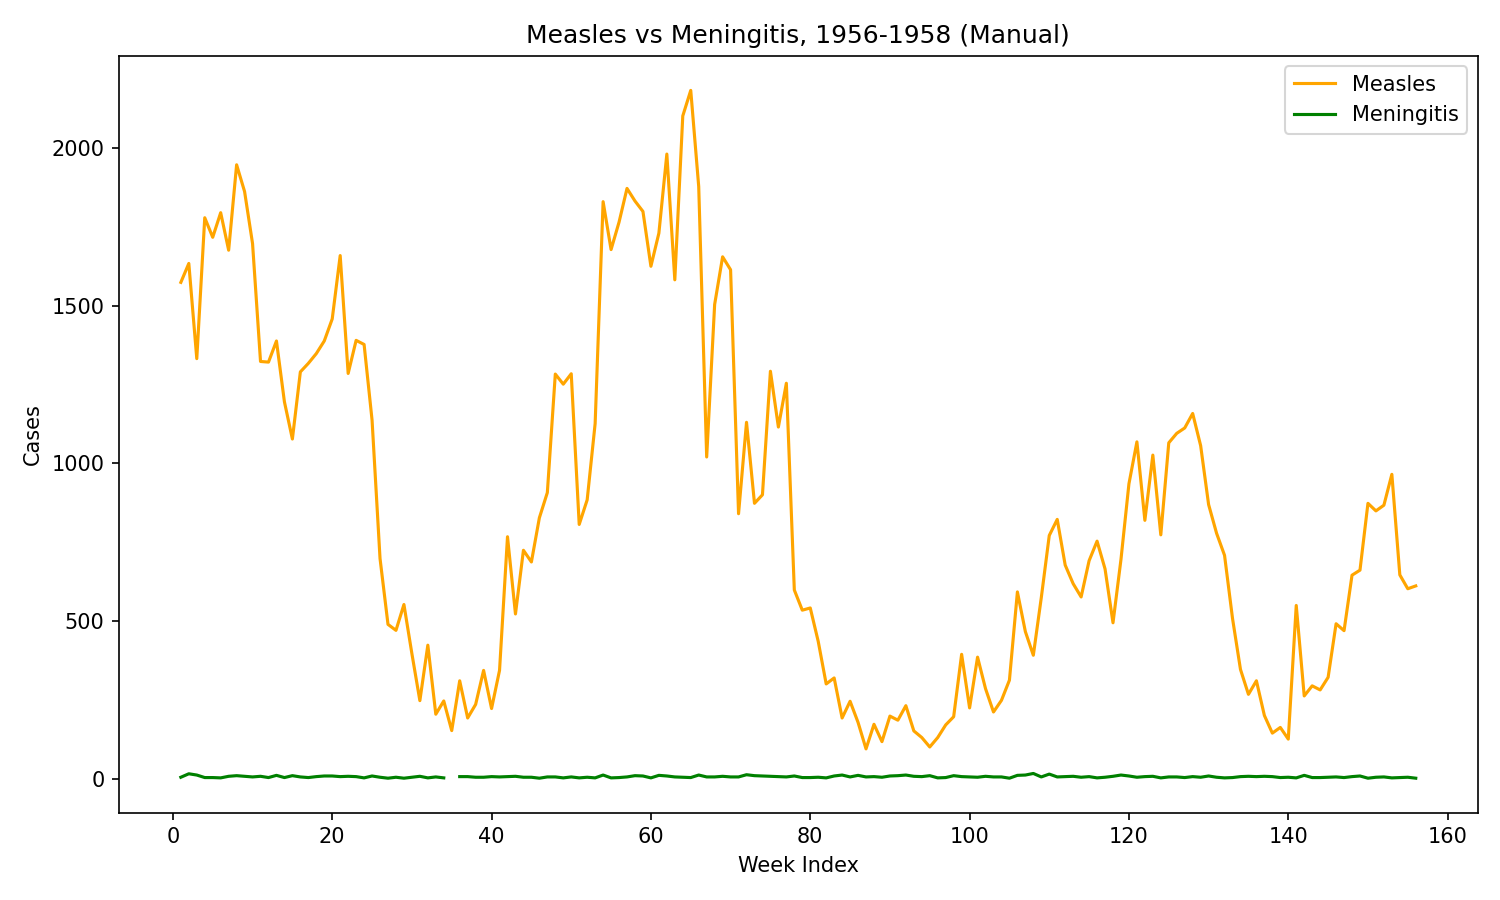
\includegraphics[width=\textwidth]{figure/measles-vs-meningitis-manual.png}
    \end{subfigure}
    \hfill
    \begin{subfigure}[b]{0.48\textwidth}
        \centering
        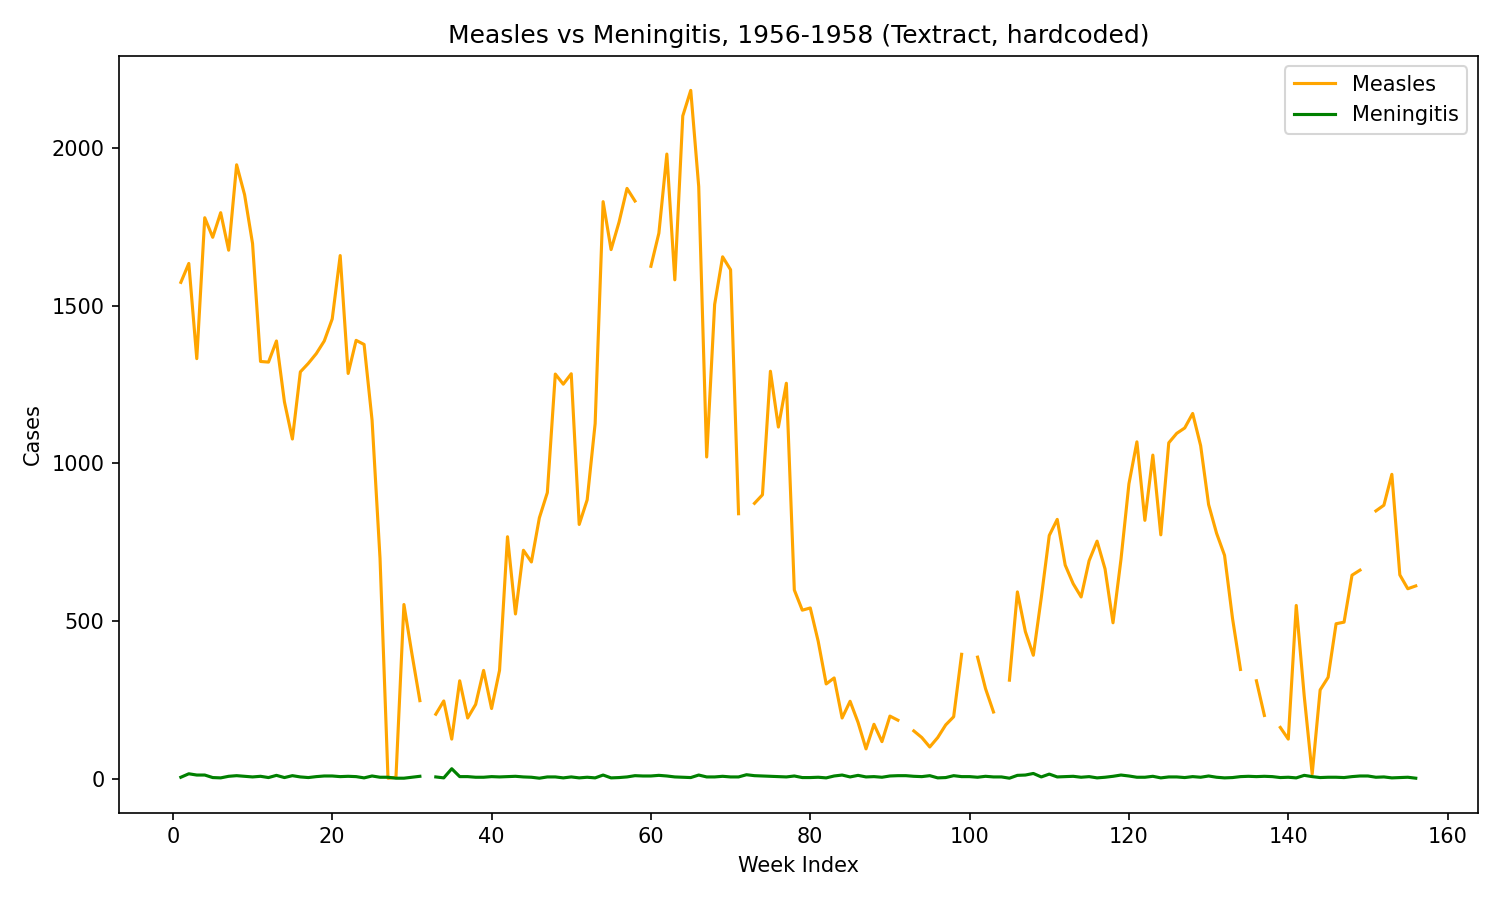
\includegraphics[width=\textwidth]{figure/measles-vs-meningitis-textract-hardcoded.png}
    \end{subfigure}
    
    \caption{Comparison of manual versus Textract disease incidence for Measles and Meningitis. Data version: manually corrected (outlier removal, \cref{sec:hardcoding}). The Meningitis data without this additional step is seen in \cref{fig:meningitiscomparison}.}
    \label{fig:comparisonIncidentsMM}
\end{figure}

The cross-correlation between Measles and Meningitis is weak across all lags in both the manual and Textract datasets, with values generally between about $-0.11$ and $0.09$ (\cref{tab:ccf_summary}). Because these correlations are close to zero throughout, this pair is the one for which a relative-difference metric was least informative: at several lags the manual correlation itself is close to zero, so any ratio against it is unstable regardless of how small the absolute discrepancy is. The manual series peaks at lag $3$ and the Textract series at lag $2$, a change in peak lag of $-1$ week; the change in peak correlation is not small in relative terms, though both values are close to zero ($0.0848$ manual vs.\ $0.1366$ Textract, a difference of $0.0517$). The largest absolute discrepancy between the two series is $0.0750$ (at lag $4$) and the root-mean-square difference is $0.0401$ -- both larger in absolute terms than the Measles/Chickenpox discrepancies above, and a relative-difference expression of this same gap would read an order of magnitude larger still, for the reason given above. Textract captures the overall cross-correlation pattern here, and the largest discrepancies occur at lags where both correlations are already small.



\begin{figure}
    \centering
    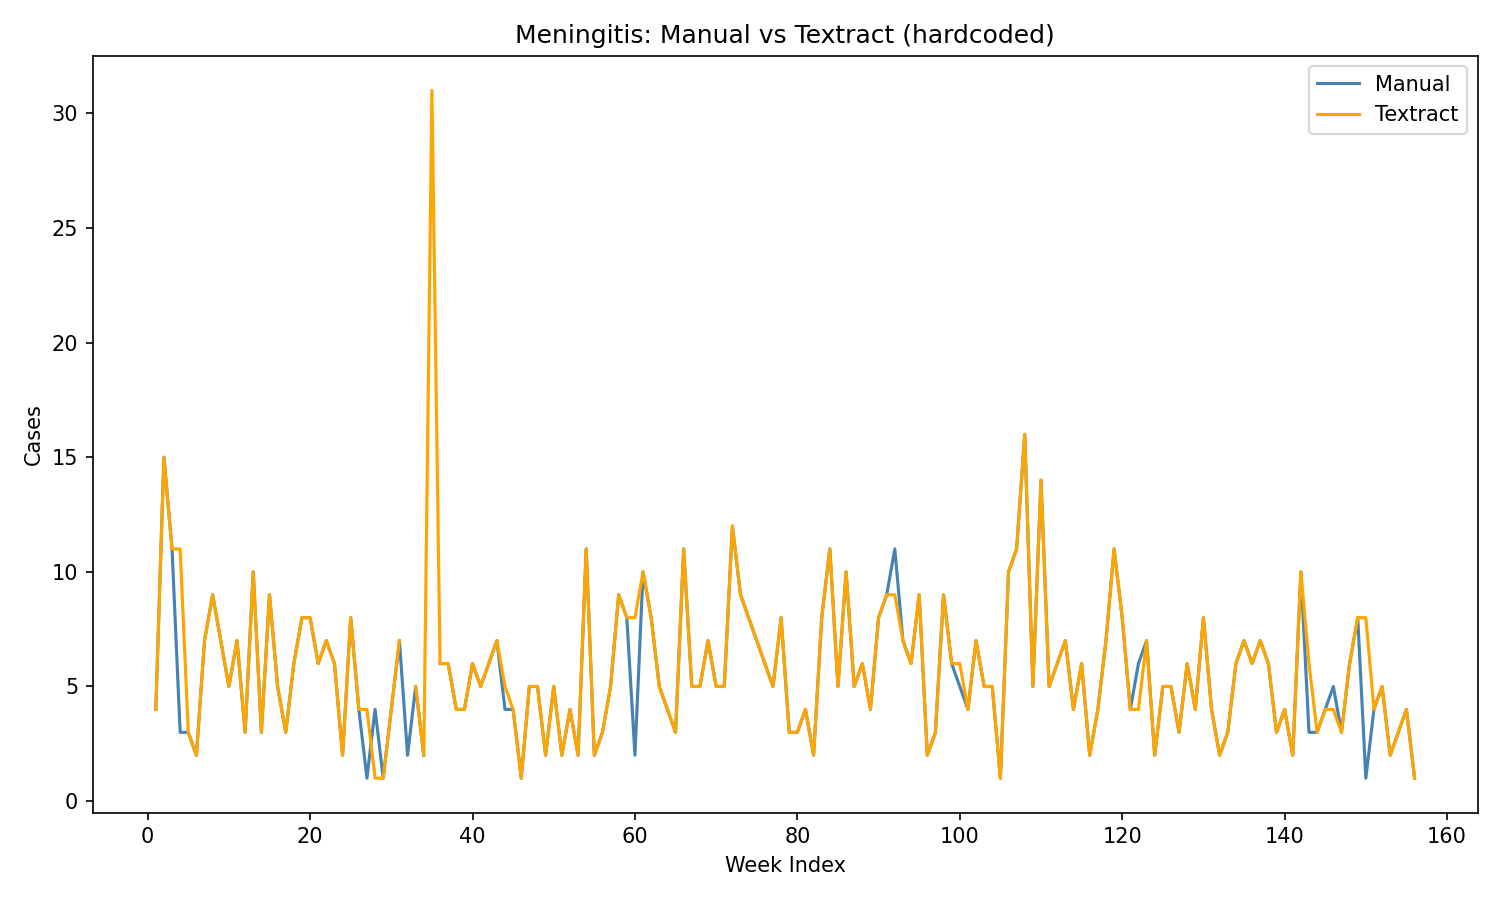
\includegraphics[width=0.5\linewidth]{figure/meningitis-manual-vs-textract.png}
    \caption{Manual (blue) and Textract (orange) time series for Meningitis. The Textract data shown here is plotted \textit{after} the additional post-processing seen in \cref{sec:hardcoding}; see \cref{tab:ccf_summary} for the quantified comparison.}
    \label{fig:meningitiscomparison}
\end{figure}



\begin{figure}[h!]
    \centering
    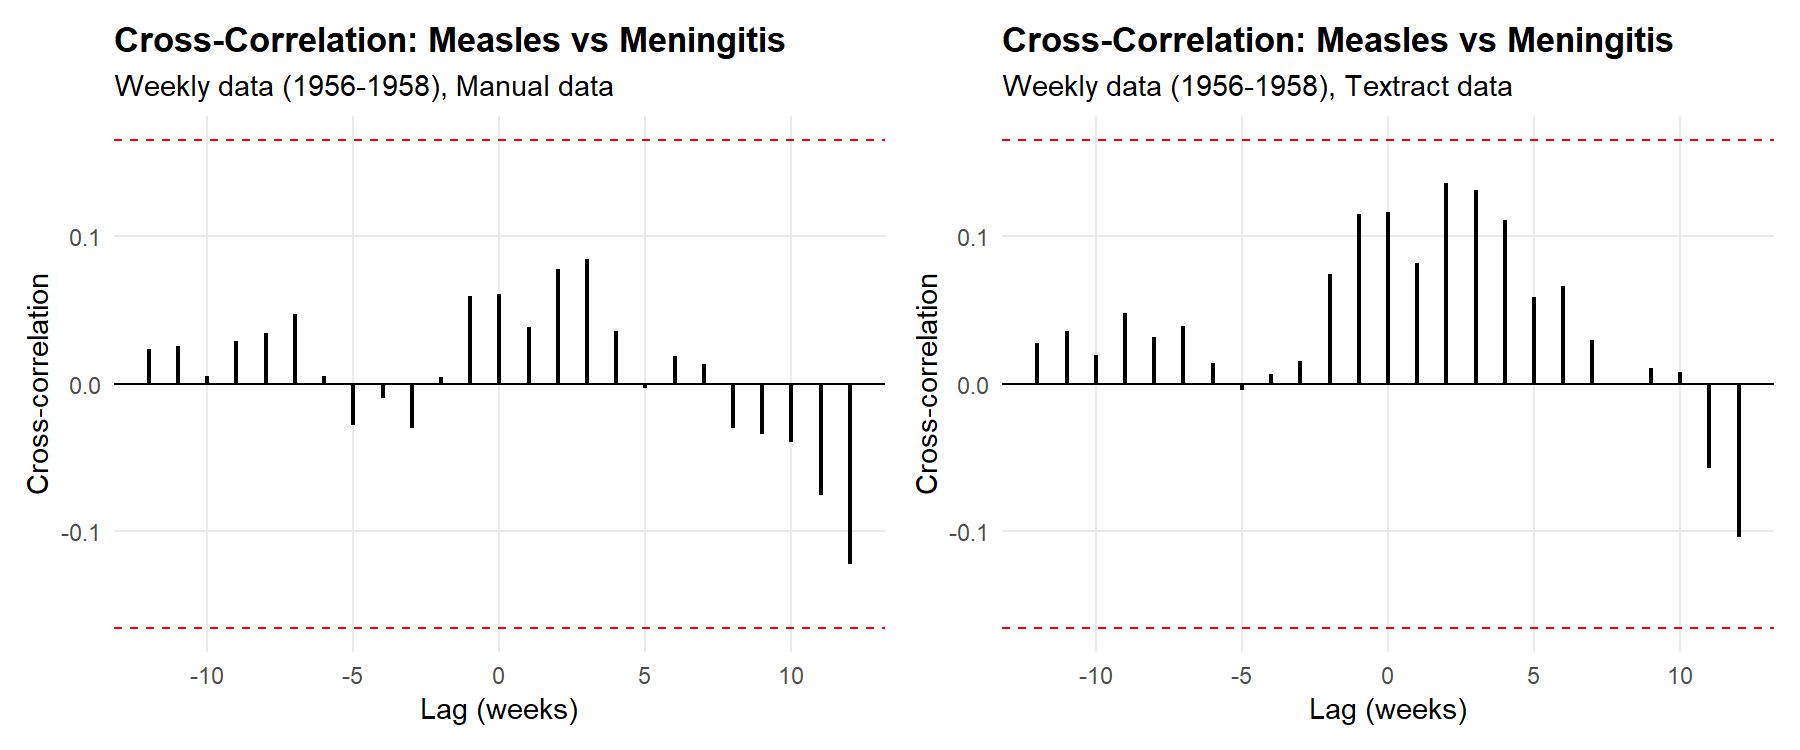
\includegraphics[width=\linewidth]{figure/fig14_measles_meningitis_ccf.png}
    \caption{Comparison of manual versus Textract disease cross-correlation for Measles and Meningitis. Data version: manually corrected (outlier removal, \cref{sec:hardcoding}). Regenerated from the corrected common-calendar-week CCF calculation (\texttt{analysis/cross\_correlation.R}); see \cref{tab:ccf_summary}.}
    \label{fig:comparisonCrossCorrelation2}
\end{figure}

Finally, the same procedure is repeated for a third pair of diseases, namely Chickenpox and Mumps. The Textract series used here are manually corrected, following the same procedure applied to the Meningitis data (\cref{sec:hardcoding}). Time series for both diseases are extracted from the manually curated dataset, and the Textract output, and the corresponding incidence curves are plotted in \cref{fig:comparisonIncidentschM}. Prior to computing the cross-correlation, the extracted data undergoes the same post-processing pipeline used for the Meningitis dataset. In particular, OCR-related errors identified as outliers are manually corrected to ensure that the resulting time series is suitable for analysis. This correction procedure is described in detail in \cref{sec:hardcoding}.


We see in \cref{fig:comparisonCrossCorrelation3} that the graphs of the cross-correlation calculated between Chickenpox and Mumps are very similar between the manual and Textract data. The summary statistics in \cref{tab:ccf_summary} (per-lag values in \hyperref[sec:supp]{Supplementary Material}, Table S3) confirm this: the differences between the two datasets at each lag are small.

\begin{figure}[h!]
    \centering
    
    \begin{subfigure}[b]{0.48\textwidth}
        \centering
        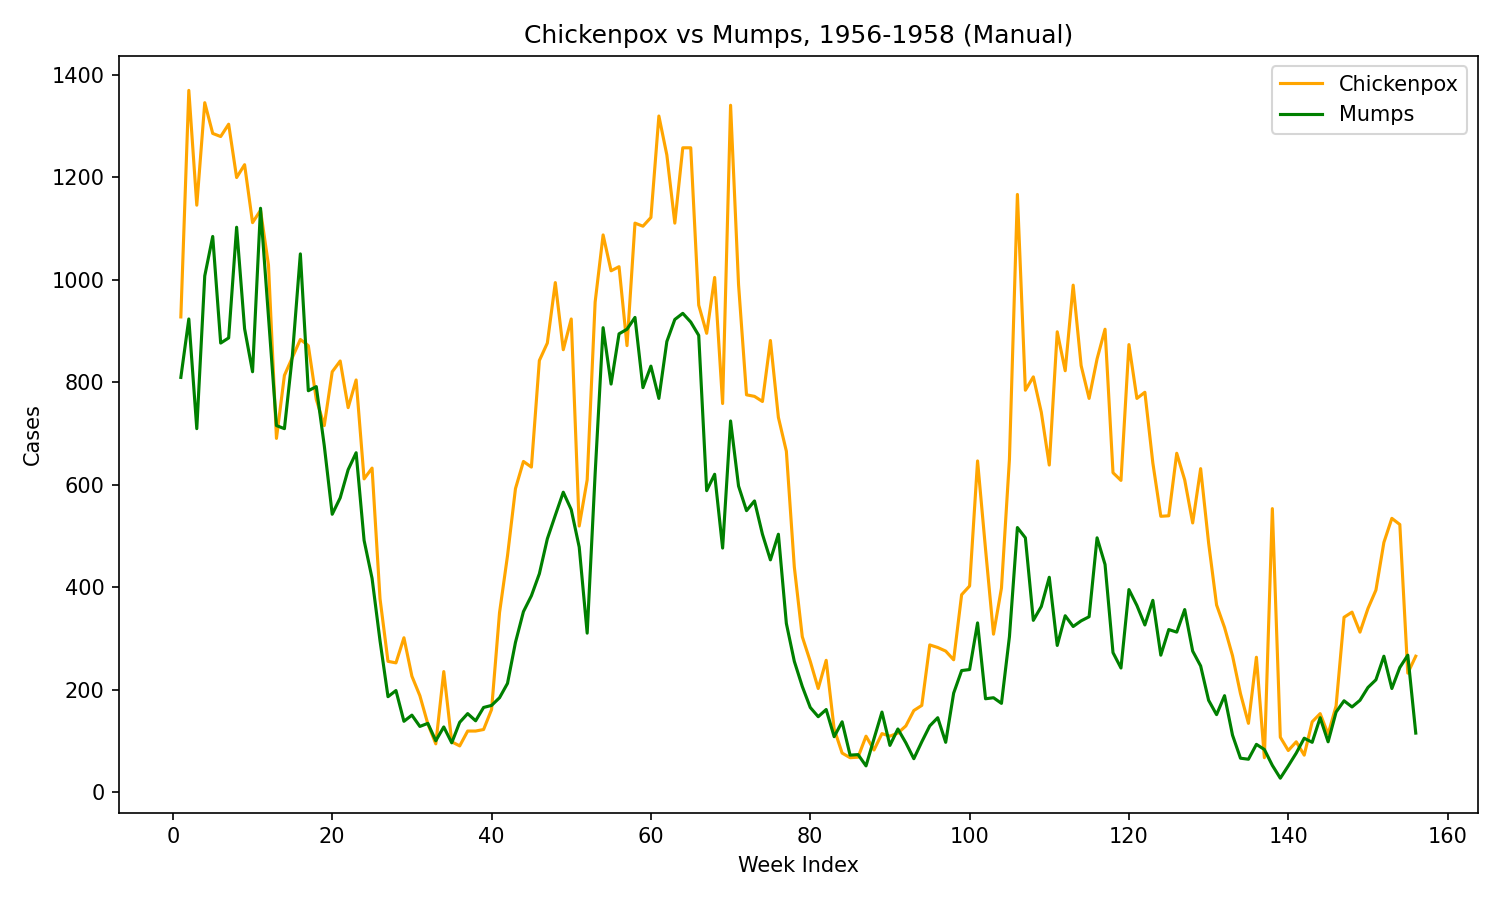
\includegraphics[width=\textwidth]{figure/manual_chickenpox_mumps.png}
    \end{subfigure}
    \hfill
    \begin{subfigure}[b]{0.48\textwidth}
        \centering
        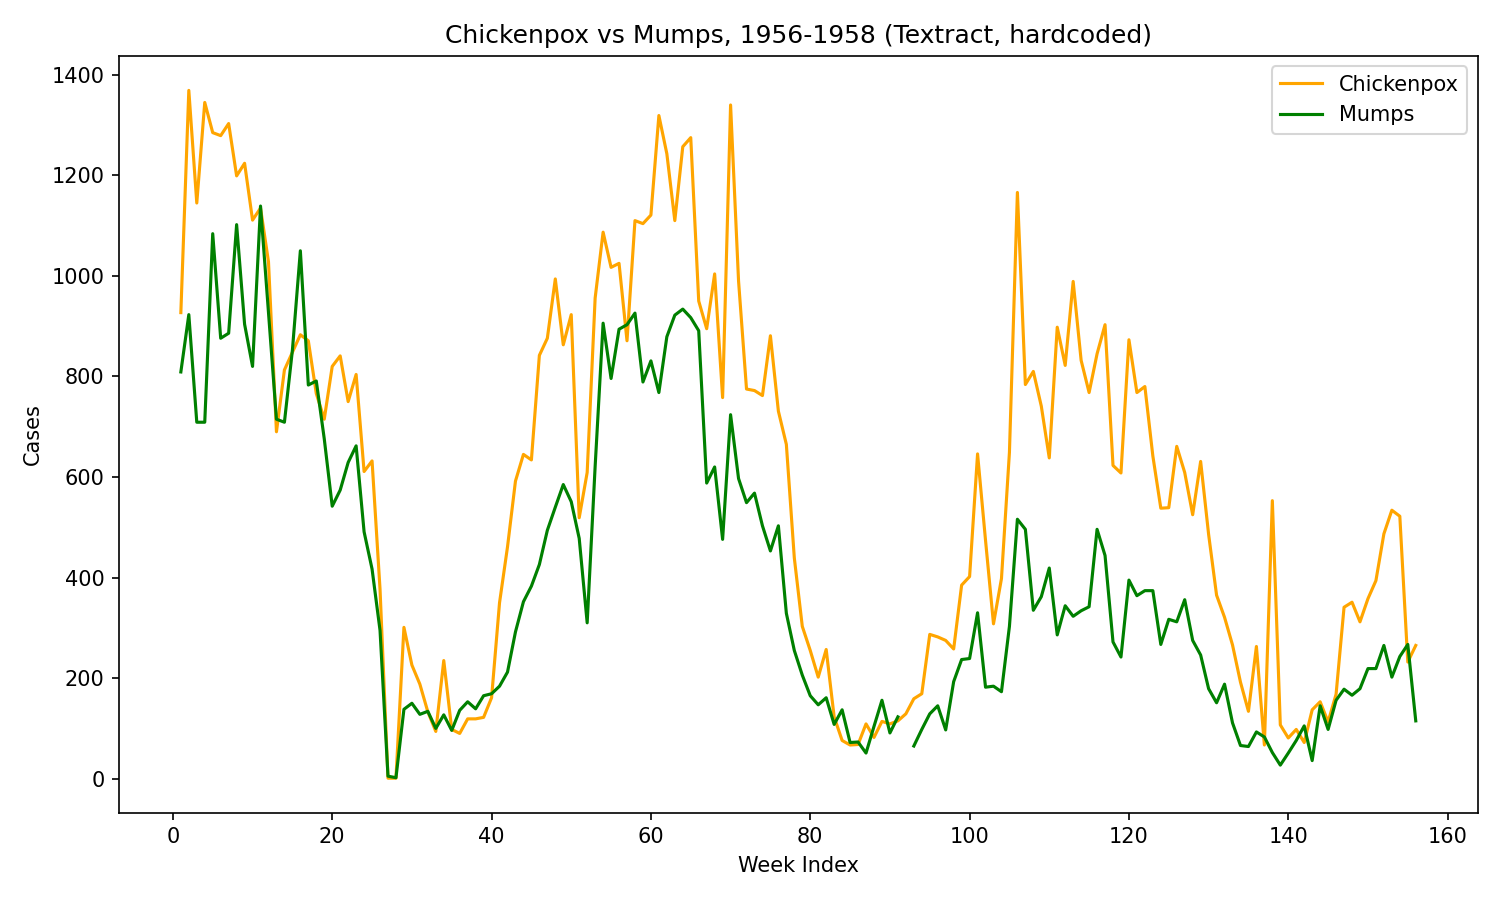
\includegraphics[width=\textwidth]{figure/textract_chickenpox_mumps_hardcoded.png}
    \end{subfigure}
    
    \caption{Comparison of manual versus Textract disease incidence for Chickenpox and Mumps. Data version: manually corrected (\cref{sec:hardcoding}).}
    \label{fig:comparisonIncidentschM}
\end{figure}

\begin{figure}[h!]
    \centering
    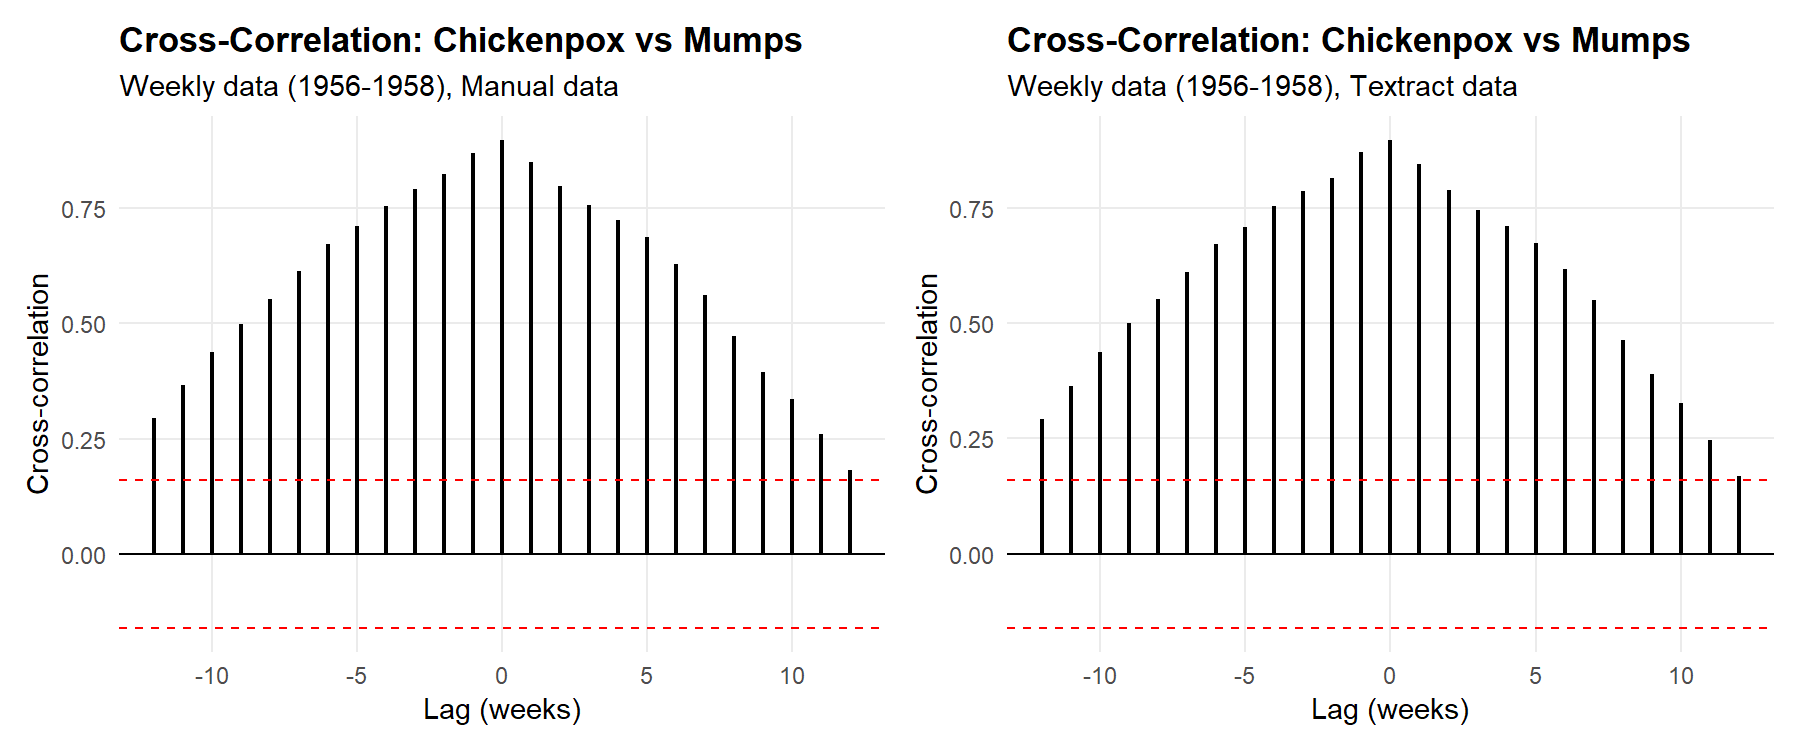
\includegraphics[width=\linewidth]{figure/fig16_chickenpox_mumps_ccf.png}
    \caption{Comparison of manual versus Textract disease cross-correlation for Chickenpox and Mumps. Data version: manually corrected (\cref{sec:hardcoding}). Regenerated from the corrected common-calendar-week CCF calculation (\texttt{analysis/cross\_correlation.R}); see \cref{tab:ccf_summary}.}
    \label{fig:comparisonCrossCorrelation3}
\end{figure}

The cross-correlation between diseases and the conclusions we draw from their CCF data are almost identical in both the manual and Textract dataset for this pair: the peak lag, which is most important for epidemiological study, is identical (lag 0 in both), the change in peak correlation is negligible ($-0.0009$), and both the largest absolute discrepancy ($0.0145$, at lag 5) and the root-mean-square difference ($0.0080$) are the smallest of the three disease pairs examined.

\Cref{tab:ccf_summary} collects these summary statistics for all three disease pairs. A strong cross-correlation near lag zero is expected for two seasonal childhood infections circulating in the same population and is not, on its own, a demanding evaluation target; what these comparisons test is whether Textract preserves the \emph{structure} of that dependence (peak lag, and the overall shape of the CCF) rather than establishing a stringent benchmark of extraction accuracy.

\begin{landscape}
\begin{table}[h]
\centering
\scriptsize
\begin{tabular}{lp{2.5cm}ccccccccc}
\toprule
Disease pair & Data version & Max $|\Delta|$ & Lag at max & RMS diff & Lag M & Lag T & $\Delta$Lag & $\rho$ M & $\rho$ T & $\Delta\rho$ \\
\midrule
Measles vs Chickenpox & processed, no manual correction & 0.0699 & 7 & 0.0376 & 0 & 0 & 0 & 0.8584 & 0.8329 & $-0.0255$ \\
Measles vs Meningitis & \textbf{manually corrected} & 0.0750 & 4 & 0.0401 & 3 & 2 & $-1$ & 0.0848 & 0.1366 & $0.0517$ \\
Chickenpox vs Mumps & \textbf{manually corrected} & 0.0145 & 5 & 0.0080 & 0 & 0 & 0 & 0.8983 & 0.8974 & $-0.0009$ \\
\bottomrule
\end{tabular}
\caption{Summary of cross-correlation agreement between manual and Textract series for all three disease pairs, computed by \texttt{analysis/ccf\_summary.py} from the per-lag CCF values (\hyperref[sec:supp]{Supplementary Material}, Tables S1--S3), which are themselves computed by \texttt{analysis/cross\_correlation.R} after merging the manual and Textract series on their shared week identifier and restricting to weeks with complete data in both sources at every lag (the two series are no longer NA-dropped independently, which previously let them cover different numbers of calendar weeks per disease pair). Lag range $k \in \{-12,\dots,+12\}$ (n = 25 lags). Sign convention: all differences are Textract $-$ Manual. ``M''/``T'' denote Manual/Textract; ``Lag M''/``Lag T'' and ``$\rho$ M''/``$\rho$ T'' are the peak lag and peak correlation for each series. Peak-lag ties (smaller $|k|$, then negative lag) did not occur for any of the three pairs. \textbf{Data version} follows \cref{tab:pipeline}: two of the three pairs (Meningitis, Mumps) use Textract series manually corrected following inspection (\cref{sec:hardcoding}); Measles vs.\ Chickenpox does not.}
\label{tab:ccf_summary}
\end{table}
\end{landscape}

\clearpage

\subsubsection{Time Series Statistics}
After isolating the time series for specific diseases in CANDID, we can find the peak heights and times. In \cref{fig:comparisonIncidents} we can see, in green, the time series for Measles. As mentioned, the Textract data is very visually similar to the manually entered data.


We report both the initial exponential growth rate $r$ and the doubling time $T_{\mathrm{d}}$ it implies for the Measles epidemics: $r$ is the quantity actually estimated by the model, and $T_{\mathrm{d}}$ is a transformation of it that is easier to interpret numerically, so reporting $T_{\mathrm{d}}$ alone would hide the scale on which the model was fitted. Both are calculated with the R package \texttt{epigrowthfit} \cite{JaganRpkg}, using the model specification given in \cref{sec:measuresAccuracy}. Because our incidence data are indexed in weeks, $r$ is a per-week rate. The graphs below show the fitted curves and doubling-time annotation for Measles for both datasets (see \cref{fig:growthratesm}).



We see in \cref{table:measles_growthrate_results} the numeric results comparing growth rate, doubling time, peak week, and smoothed peak incidence between the manually entered and automated datasets.

\begin{figure}[h!]
    \centering
    
    \begin{subfigure}[b]{0.48\textwidth}
        \centering
        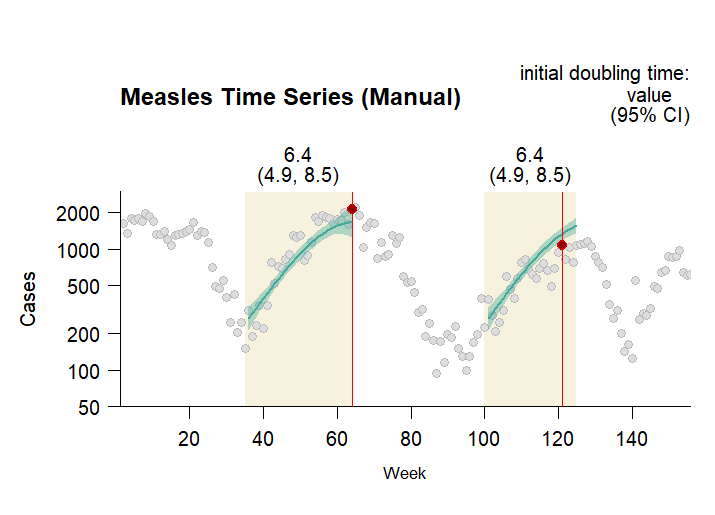
\includegraphics[width=\textwidth]{figure/growthratesmanual.png}
    \end{subfigure}
    \hfill
    \begin{subfigure}[b]{0.48\textwidth}
        \centering
        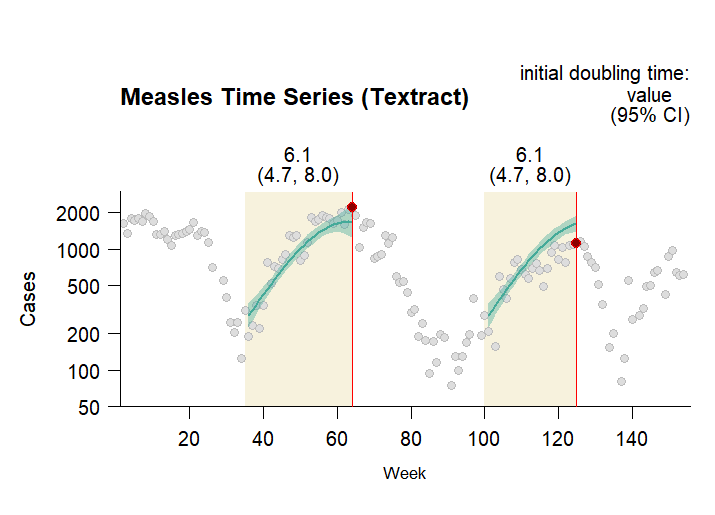
\includegraphics[width=\textwidth]{figure/growratestextract.png}
    \end{subfigure}
    
    \caption{Manual versus Textract Measles growth rates as described in
    \cref{sec:measuresAccuracy}. Data version: processed Textract data (\cref{tab:pipeline}, Stage 2), without manual correction. Shaded bands mark the two fitting windows (week 35--64 and week 95--126). The annotated ``initial doubling time: value (95\% CI)'' is in weeks and is the same number in both shaded windows for a given panel: this is not a labelling error but a direct consequence of the model specification (\cref{sec:measuresAccuracy}), which estimates one growth rate shared across both windows rather than a separate rate per window; see \cref{table:measles_growthrate_results} for the corresponding growth rate $r$.}
    \label{fig:growthratesm}
\end{figure}

\begin{table}[h]
\centering
\small
\resizebox{\textwidth}{!}{%
\begin{tabular}{lccccccccc}
\toprule
\textbf{Window} & \textbf{Fit range (wk)} & \textbf{n obs} & \textbf{Source} & \textbf{Peak week} & \textbf{Smoothed peak incidence} & \textbf{$\Delta$ week} & \textbf{$\Delta$ cases (\%)} & \textbf{$r$ (wk$^{-1}$, 95\% CI)} & \textbf{$T_{\mathrm{d}}$ (wk, 95\% CI)} \\
\midrule
\multirow{2}{*}{Window 1} & \multirow{2}{*}{35--64} & 30 & Manual   & 64  & 1967 & --   & --            & 0.137 (0.114, 0.165)  & 5.1 (4.2, 6.1) \\
                          &                          & 30 & Textract & 64  & 2161 & 0    & $+194$ ($+9.84$) & 0.124 (0.100, 0.154)  & 5.6 (4.5, 6.9) \\
\midrule
\multirow{2}{*}{Window 2} & \multirow{2}{*}{95--126} & 32 & Manual   & 126 & 1040 & --   & --             & 0.137 (0.114, 0.165)  & 5.1 (4.2, 6.1) \\
                          &                          & 30 & Textract & 126 & 1174 & 0    & $+134$ ($+12.91$) & 0.124 (0.100, 0.154)  & 5.6 (4.5, 6.9) \\
\bottomrule
\end{tabular}%
}
\caption{Comparison of peak week, smoothed peak incidence, growth rate, and doubling time between Textract and manual data for Measles, recomputed from \texttt{data/analysis\_intermediates/table4\_measles\_peak\_comparison.csv} and \texttt{growth\_rate\_summary.csv} (\texttt{analysis/growthrates.R}). Data version: processed Textract data (\cref{tab:pipeline}, Stage 2), without manual correction -- the only Textract version available for Measles (see \cref{sec:NDD}). Sign convention: $\Delta$ = Textract $-$ Manual. Peaks are located from a LOESS-smoothed series within each fit window (peak-detection rule, \cref{sec:measuresAccuracy}); ties resolve to the earliest week. $n$ obs is 30 for every window/source except Manual Window 2 (32); the Textract series is missing 2 weeks (weeks 98 and 102) inside Window 2, which is why the Manual and Textract fits for that window are not run on identical $n$. $r$ and $T_{\mathrm{d}}$ are estimated from a single growth-rate parameter shared across both fitting windows (model specification, \cref{sec:measuresAccuracy}) and are therefore identical for Window 1 and Window 2 within a given source; both fits converged (\texttt{optim} status ``relative convergence''). The Manual/Textract 95\% CIs for $r$ overlap and each point estimate falls within the other source's CI (\cref{sec:NDD}); this comparison is not on strictly identical $n$ given the two missing Textract weeks noted above.}
\label{table:measles_growthrate_results}
\end{table}


\begin{figure}[h!]
    \centering
    
    \begin{subfigure}[b]{0.48\textwidth}
        \centering
        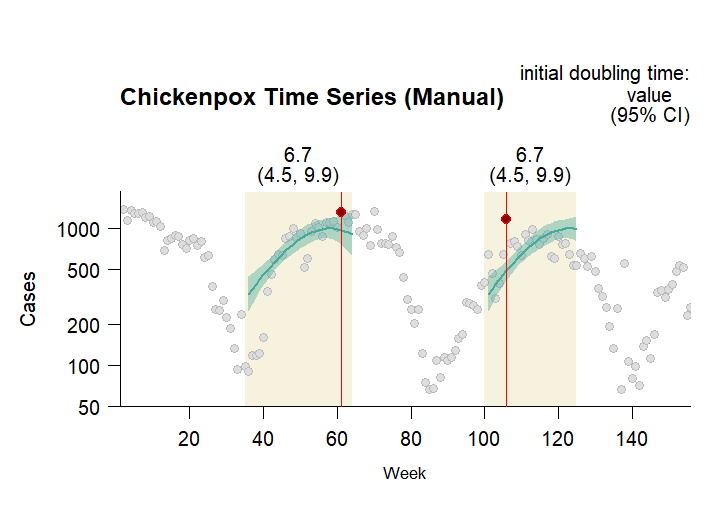
\includegraphics[width=\textwidth]{figure/chickenpox_growth_rate_manual.png}
    \end{subfigure}
    \hfill
    \begin{subfigure}[b]{0.48\textwidth}
        \centering
        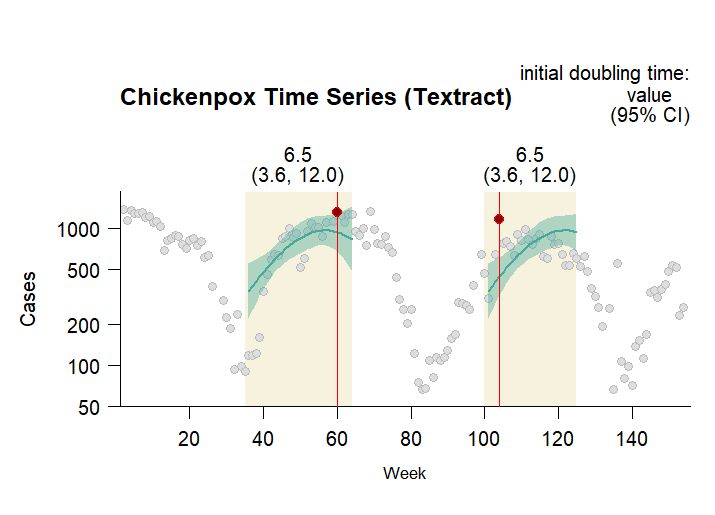
\includegraphics[width=\textwidth]{figure/chickenpox_growth_rate_textract.png}
    \end{subfigure}
    
    \caption{Manual versus Textract Chickenpox growth rates as described in
    \cref{sec:measuresAccuracy}. Data version: processed Textract data (\cref{tab:pipeline}, Stage 2), without manual correction. Shaded bands mark the two fitting windows (week 35--64 and week 95--126). The annotated ``initial doubling time: value (95\% CI)'' is in weeks and is the same number in both shaded windows for a given panel: this is not a labelling error but a direct consequence of the model specification (\cref{sec:measuresAccuracy}), which estimates one growth rate shared across both windows rather than a separate rate per window; see \cref{tab:growthrateschickenpox} for the corresponding growth rate $r$.}
    \label{fig:growthrateschickenpox}
\end{figure}


\begin{table}[h]
\centering
\small
\resizebox{\textwidth}{!}{%
\begin{tabular}{lccccccccc}
\toprule
\textbf{Window} & \textbf{Fit range (wk)} & \textbf{n obs} & \textbf{Source} & \textbf{Peak week} & \textbf{Smoothed peak incidence} & \textbf{$\Delta$ week} & \textbf{$\Delta$ cases (\%)} & \textbf{$r$ (wk$^{-1}$, 95\% CI)} & \textbf{$T_{\mathrm{d}}$ (wk, 95\% CI)} \\
\midrule
\multirow{2}{*}{Window 1} & \multirow{2}{*}{35--64} & 30 & Manual   & 64  & 1223 & --   & --           & 0.144 (0.125, 0.167) & 4.8 (4.2, 5.5) \\
                          &                          & 30 & Textract & 64  & 1313 & 0    & $+90$ ($+7.42$) & 0.144 (0.108, 0.193) & 4.8 (3.6, 6.4) \\
\midrule
\multirow{2}{*}{Window 2} & \multirow{2}{*}{95--126} & 32 & Manual   & 114 & 882  & --   & --           & 0.144 (0.125, 0.167) & 4.8 (4.2, 5.5) \\
                          &                          & 32 & Textract & 112 & 882  & $-2$ & $0$ ($0.00$)    & 0.144 (0.108, 0.193) & 4.8 (3.6, 6.4) \\
\bottomrule
\end{tabular}%
}
\caption{Comparison of peak week, smoothed peak incidence, growth rate, and doubling time for Chickenpox between Textract and manual data, recomputed from \texttt{data/analysis\_intermediates/table5\_chickenpox\_peak\_comparison.csv} and \texttt{growth\_rate\_summary.csv} (\texttt{analysis/growthrates.R}). Data version: processed Textract data (\cref{tab:pipeline}, Stage 2), without manual correction -- the only Textract version available for Chickenpox (see \cref{sec:NDD}). Sign convention: $\Delta$ = Textract $-$ Manual. Peaks are located from a LOESS-smoothed series within each fit window (peak-detection rule, \cref{sec:measuresAccuracy}); ties resolve to the earliest week. $r$ and $T_{\mathrm{d}}$ are estimated from a single growth-rate parameter shared across both fitting windows and are therefore identical for Window 1 and Window 2 within a given source; both fits converged. The Manual/Textract 95\% CIs for $r$ overlap and each point estimate falls within the other source's CI (\cref{sec:NDD}); note the Textract CI is noticeably wider than the Manual CI (0.108--0.193 vs.\ 0.125--0.167).}
\label{tab:growthrateschickenpox}
\end{table}

We can compare these same statistics with a different disease. For example, \cref{fig:growthrateschickenpox} showcases the doubling times and peaks for Chickenpox as seen in the manual and extracted versions of the dataset. These statistics are compared in \Cref{tab:growthrateschickenpox}.

Peak week is unchanged (Textract $-$ Manual $= 0$) in three of the four windows, and differs by $-2$ weeks in the fourth (Chickenpox, Window 2); smoothed peak incidence differs by up to $+194$ cases (Measles Window 1, $+9.84\%$) in absolute terms and by up to $+12.91\%$ (Measles Window 2, $+134$ cases) in relative terms -- the largest absolute and largest relative discrepancies fall in different windows -- with Textract consistently over-counting relative to Manual across all four windows. None of the four reported peak weeks can be cross-checked against the row-sum validation of \cref{sec:hardcoding}, since that validation covers only 1956 while all four peaks fall in 1957--1958 (\cref{sec:measuresAccuracy}).

For the growth rate itself: the Measles estimate is $r = 0.137$ wk$^{-1}$ (95\% CI 0.114--0.165) from the manual series and $r = 0.124$ wk$^{-1}$ (95\% CI 0.100--0.154) from Textract, a difference of $\Delta r = -0.013$ wk$^{-1}$; the corresponding doubling times are 5.1 (4.2, 6.1) and 5.6 (4.5, 6.9) weeks, $\Delta T_{\mathrm{d}} = +0.5$ weeks. For Chickenpox, $r = 0.144$ wk$^{-1}$ from both sources to three significant figures (95\% CI 0.125--0.167 manual, 0.108--0.193 Textract), $\Delta r \approx -0.0004$ wk$^{-1}$; doubling times are 4.8 (4.2, 5.5) and 4.8 (3.6, 6.4) weeks, $\Delta T_{\mathrm{d}} = +0.01$ weeks. In both diseases the Manual and Textract 95\% CIs for $r$ overlap, and each point estimate falls inside the other source's interval; the Chickenpox Textract CI is also visibly wider than its Manual counterpart, which is expected given no more data points were available to the fit (\crefrange{table:measles_growthrate_results}{tab:growthrateschickenpox} report $n$ observations per window). The fitted early-growth rates were similar in these two selected comparisons: the estimated Textract-minus-manual differences were $\Delta r = -0.013$ wk$^{-1}$ for Measles and $\Delta r \approx -0.0004$ wk$^{-1}$ for Chickenpox. Overlapping confidence intervals are reported here as a descriptive feature of the two fits, not as a statistical test of equivalence; this observation is scoped to the two diseases (Measles, Chickenpox) and two epidemic windows examined here, and it does not establish that growth-rate estimation from Textract data is reliable in general.


\subsection{Remarks on Dataset Specific Coding}\label{sec:hardcoding}

Several challenges arose when computing row-wise sums for each disease. The primary issue was the extraction errors, such as row misalignment or mislabeled diseases. These issues shifted entire rows of values and consistently propagated across tables, making it difficult to associate values with the correct disease directly. For example, if a disease name contains a comma in the original table, Textract extracts this as two separate cells, shifting the following disease incidence values. As each table has the same or similar disease names, this problem in extraction appeared in each table corresponding to that row. 

Grouping entries by disease (rather than by week as extracted) before performing the summation reduced this complexity. This limited the need for extensive manual intervention, as most diseases had identical errors in each table.

When a shift occurred (typically due to errors in disease labels) the position of the reported total and its corresponding contributing values became offset, and the indices used to identify these values were no longer valid. To address this, the correct indices were re-identified through manual inspection of the extracted data for each disease, and the summation inputs were adjusted accordingly.

An example of this shifting in CANDID occurs with Scarlet Fever. Persistent discrepancies were observed between reported and recomputed sums. Beginning in week 5 of 1956, all row sums appeared incorrect. Investigation revealed that the disease label had changed from ``Scarlet Fever'' to ``Scarlet Fever, etc.'' in the original document. The introduction of a comma altered the table parsing, causing a shift in all subsequent cell values within the row. This shift propagated through the extraction, leading to misalignment. Resolving this issue required manually identifying the change and recombining the affected cell values to restore the correct structure.

A further consideration in the row-sum computation is the structure of the original tables: a row index is printed both at the beginning of each row and repeated at the end (see \cref{fig:NDD1}), and the province ``Report Week'' values are not the only numeric-looking entries in the row. Rather than iterating generically across the row and attempting to filter out non-contributing values at runtime, the row-sum script (\texttt{analysis/row\_sum\_check.py}) avoids this problem by construction: it reads the Canada report-week total from a fixed column and sums only the fixed set of columns, identified directly from the table layout in \cref{fig:NDD1}, that hold each province's report-week value (\cref{fig:hardcode}). Because the contributing columns are specified explicitly rather than inferred from cell content, the row index and any other non-contributing cell are never candidates for inclusion in the sum.



\begin{figure}[h]
\centering
\begin{lstlisting}[language=Python]
TARGET_COL = 2
CONTRIB_COLS = list(range(8, 36, 3))  # 8, 11, 14, ..., 35 -- one per province

target = to_int_or_none(row[TARGET_COL])
contributors = [(c, to_int_or_none(row[c])) for c in CONTRIB_COLS]
computed = sum(v for _, v in contributors if v is not None)
\end{lstlisting}
\caption{The column layout used by the row-sum validation script (\texttt{analysis/row\_sum\_check.py}) to identify the Canada report-week total (column 2) and each province's contributing report-week value (columns 8, 11, 14, \ldots, 35, one per province at three-column intervals), as reproduced from the actual script rather than paraphrased.}
\label{fig:hardcode}
\end{figure}
 
We also had to correct extraction errors when comparing the epidemiological statistics between the two datasets. The extracted Meningitis time series contains errors that appear as large, isolated spikes, which are not consistent with the expected disease patterns. Because these errors would distort the results of the cross-correlation analysis, they were corrected before proceeding.
The unprocessed time series for Measles and Meningitis is shown in \cref{fig:rawMeningitisTextract}. The Measles data follows a smooth and expected pattern, while the Meningitis data includes several sharp spikes that do not match the original dataset. These spikes are caused by OCR errors, where some values are misread or incorrectly extracted.

The following is another example of the Textract time series for Mumps versus Chickenpox, before our manual correction (see \cref{fig:mumpsraw}).

\begin{figure}[H]
    \centering
    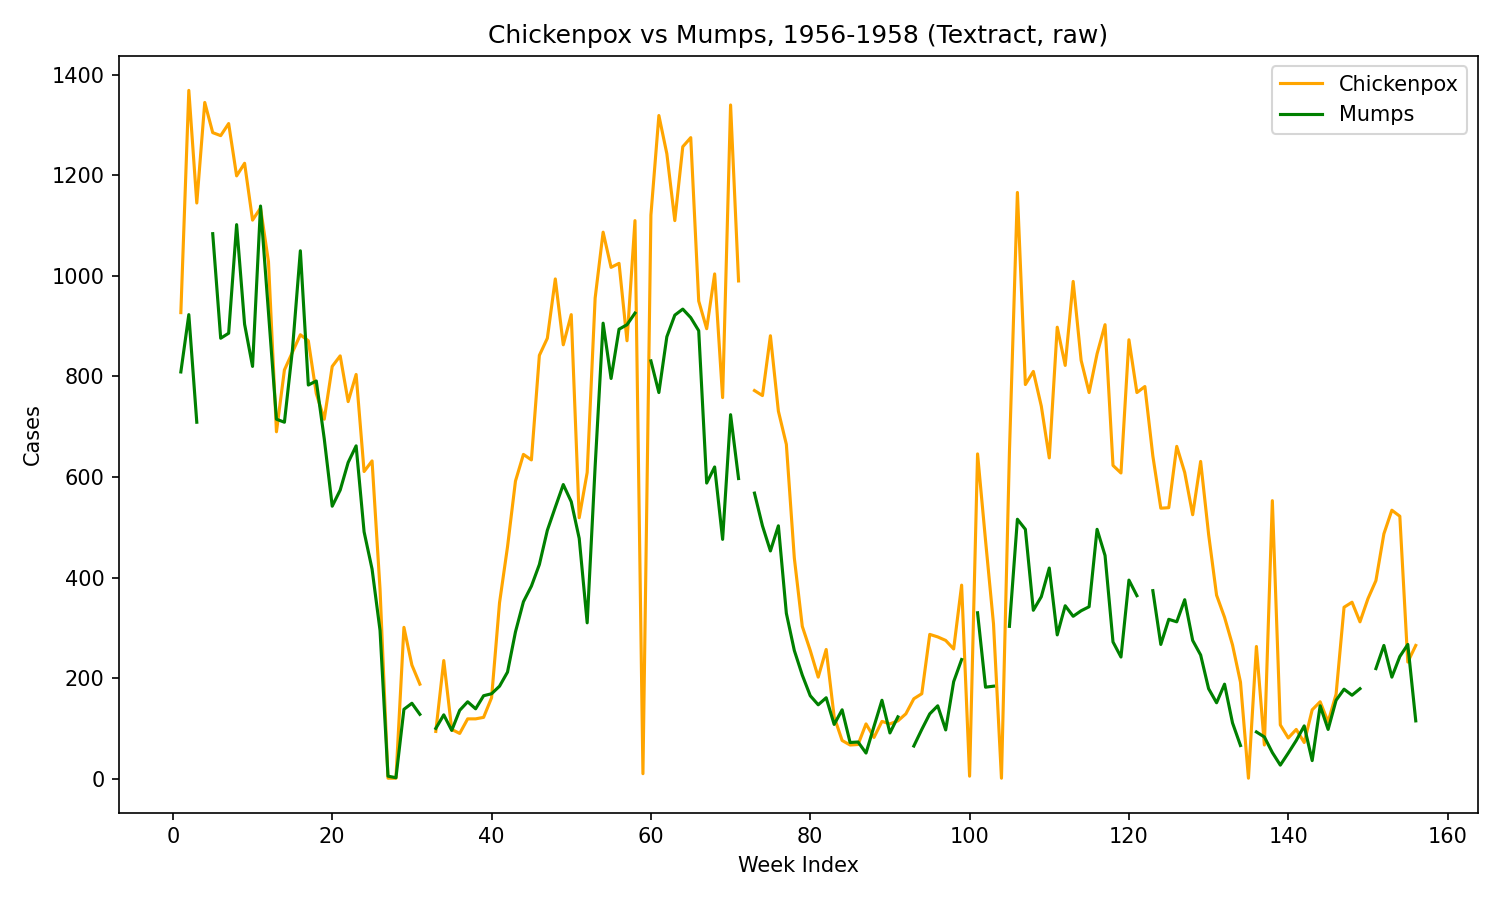
\includegraphics[width=0.7\linewidth]{figure/textract_chickenpox_mumps.png}
    \caption{Data version: raw/uncorrected Textract values (prior to the manual correction in \cref{sec:hardcoding}). The time series for Chickenpox and Mumps from Textract, with clear errors seen around weeks 60, 100, 110, etc as well as missing values.}
    \label{fig:mumpsraw}
\end{figure}


Although these errors are large, they occur only occasionally: a small number of spikes were identified across the affected time series. We identified them using a boxplot or violin plot (see \cref{fig:menboxplot}), which highlights these extreme values compared to the rest of the data. This method identified the extreme values in our data.

Correcting these incidence values by checking against the original dataset took less than 20 minutes for the Meningitis and Mumps series reviewed here (three years of weekly data). This is a measured correction time for these specific series, not an estimate of total post-processing effort across the full dataset.

\begin{figure}[H]
    \centering
    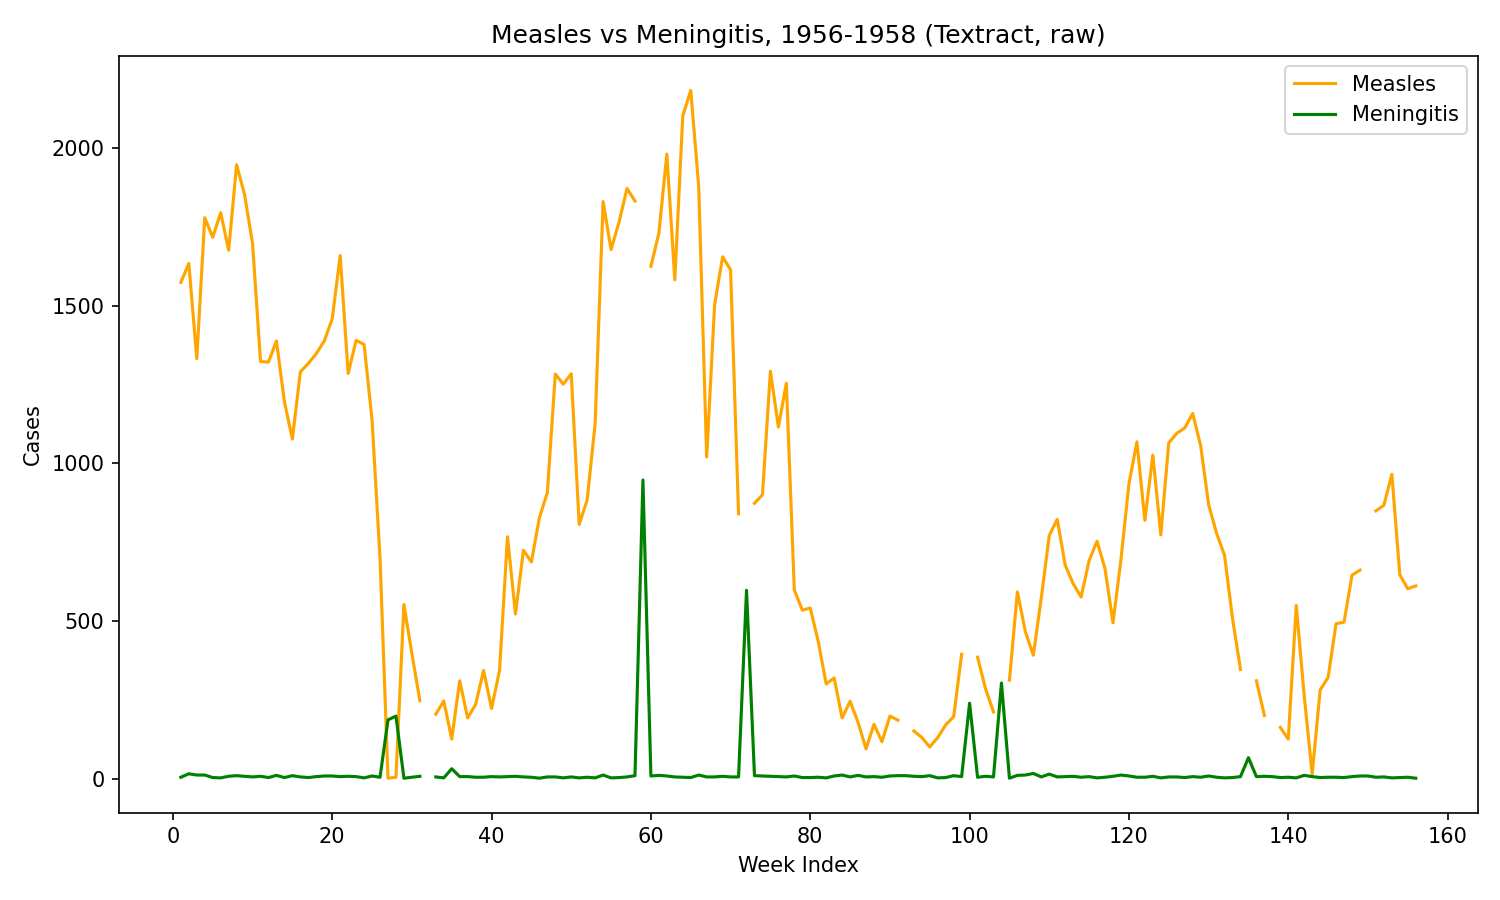
\includegraphics[width=0.5\linewidth]{figure/measles-vs-meningitis-no-hardcoding.png}
    \caption{Data version: raw/uncorrected Textract values (prior to the manual correction in \cref{sec:hardcoding}), showing clear errors in the meningitis cases.}
    \label{fig:rawMeningitisTextract}
\end{figure}

\begin{figure}[h!]
    \centering
    
    \begin{subfigure}[b]{0.48\textwidth}
        \centering
        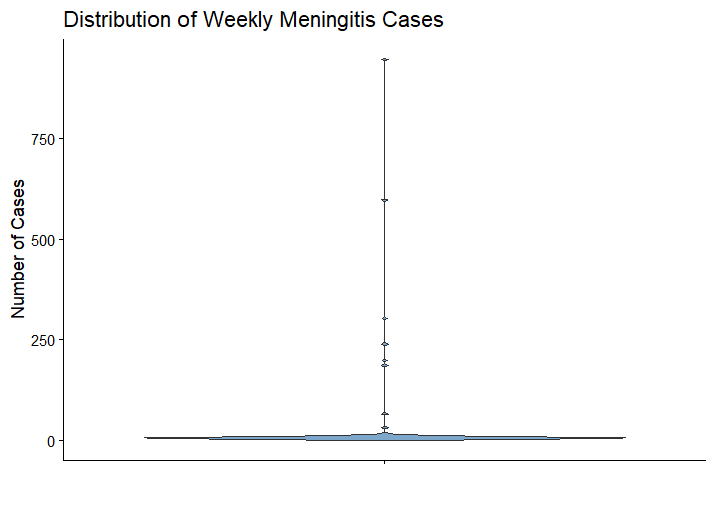
\includegraphics[width=\textwidth]{figure/violin_meningitis.png}
    \end{subfigure}
    \hfill
    \begin{subfigure}[b]{0.48\textwidth}
        \centering
        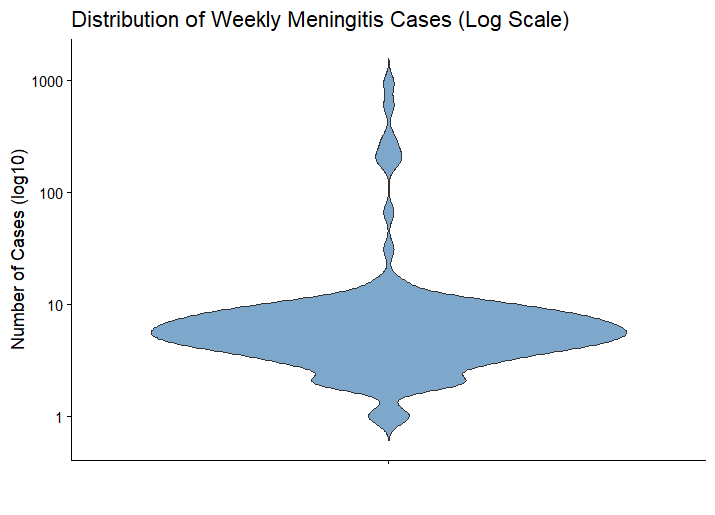
\includegraphics[width=\textwidth]{figure/violin_meningitis_log.png}
    \end{subfigure}
    
    \caption{Violin plots of Textract Meningitis data shown on linear (left) and log (right) scales.}
    \label{fig:menboxplot}
\end{figure}





\clearpage

\section{Discussion}


\subsection{Impact}\label{sec:impact}
From the perspective of epidemiology researchers, automating tabular data entry is a major aid in studying historical data. It accelerates the processing of large datasets and frees effort and resources for interpretation rather than manual transcription. Because historical sources are often vast, messy, and inconsistent, automation makes it possible to standardize and analyze them at scale, revealing patterns and insights that would have been implausible to uncover in the same amount of time with only manual data entry. The conclusions in this paper are limited to printed, regularly formatted CANDID tables from 1956--1958 processed by the specific extraction and post-processing workflow described above; we do not claim these results generalize to handwritten documents, irregularly formatted tables, or other data-extraction tools or model versions.

For an automation tool to successfully improve and accelerate the data entry process, it must meet all or most of the requirements we have set in this paper. That is, the software must be relatively simple to use and produce a dataset that is either 
\begin{enumerate}
    \item Close to the original dataset or
    \item Easy to process and fix the errors it produces
\end{enumerate}
If too much human correction is necessary, the time saved becomes relatively small, so the tool is not successful. As well, even with modest time saving, data correction is a less pleasant task for humans than data entry. In our own preliminary exploration (\hyperref[sec:supp]{Supplementary Material}, S5 Text), the conversational model we tried before Textract produced errors prevalent and tedious enough to fix that we abandoned it in favour of a tool purpose-built for table extraction.

In comparison, the errors present in Textract's table extraction are shown to be of a different character than typical manual entry errors. Textract's errors are often either small (differing from the reference value by one or two characters, with a small influence on various statistical tests on the dataset) or large. This second, large-magnitude type of error is relatively rare and occurs specifically in the extraction of disease-name string values (\cref{sec:levdist}).

Beyond the initial technical hurdle of utilizing AWS Textract programmatically, as well as the unique post-processing necessary for each dataset, the overall time and effort necessary to recreate CANDID with Textract appears to be reduced in comparison to manual data entry. Similar tables (in both size and complexity) took on average 30 minutes to fully digitize from a scanned copy by a member of McMaster's Theoretical Biology group; extrapolated at that single operator's rate to all 156 tables from 1956 to 1958, manual data entry would take an estimated 78 hours. This is not a measurement of the full manual process, but an extrapolation from one operator's rate on comparable tables. On the automated side, the components we directly measured are: script runtime ($\approx15$ minutes) and the correction pass (see \cref{sec:hardcoding}, $<20$ minutes for the reviewed series). Script development time and the remaining post-processing time were not measured. With these caveats, extraction runtime for similar tables was short relative to the extrapolated manual-entry estimate, but total person-time -- including script development and the remaining post-processing beyond the reviewed correction pass -- was not measured.

Because document-extraction systems are evolving rapidly, these findings should be understood as an evaluation of one service and workflow on one historical archive, not as a recommendation of Textract for new digitisation projects. Researchers should benchmark currently available tools on representative pages and independently audit both table structure and cell contents before selecting a workflow.



\subsection{Limitations}\label{sec:limitations}

\paragraph{No adjudicated reference standard.} The manual transcription is used throughout this paper as the comparison basis without independent re-adjudication: there was no double transcription and no two-reviewer resolution of discordant cells. The paper itself demonstrates that this reference can be wrong -- the Week 9 Measles total (\cref{sec:NDD}), where the source scan supports \textit{1882} and the reference transcription records \textit{1862}. Reported disagreement counts therefore conflate extraction errors with transcription errors, and the direction of this bias is unknown: some fraction of the cells we count as Textract errors may instead be reference-transcription errors, and vice versa. Resolving this would require two independent reviewers adjudicating a random validation sample against the source scans, with inter-reviewer agreement documented; this was not done for this paper.

A further limitation concerns data leakage in the development of our normalization and structural-repair rules. The comma/whitespace normalization, header-exclusion, and adjacent-cell content tolerance rules described in \cref{sec:simple} (see \cref{tab:pipeline}) were developed, tuned, or validated while the reference transcription was visible to us; no held-out test set of unseen tables was used. Specific instances of this include the adjacent-cell content tolerance rule (\cref{sec:postprocessing}), the Scarlet Fever comma fix (\cref{sec:hardcoding}), the fixed-column row-sum computation that avoids the repeated row index by construction (\cref{sec:hardcoding}), and the Meningitis/Mumps spike correction (\cref{sec:hardcoding}). Because these rules were shaped by the specific errors we observed in this dataset, the reported agreement figures should be read as an upper bound on the performance we would expect on previously unseen CANDID tables or other datasets, rather than as an estimate of out-of-sample accuracy.

\paragraph{Evaluation year.} Cell-level agreement (\cref{sec:simple}--\cref{sec:levdist}) covers 1956 only (52 of the 156 tables); the downstream epidemiological statistics (\cref{sec:NDD}) use all three years, 1956--1958. This is stated where the relevant numbers are first reported, but is worth naming explicitly as a limitation: the peak weeks reported in the growth-rate tables (weeks 64, 112, 114, and 126) sit entirely outside the range for which cell-level agreement was directly measured, so their accuracy rests on the assumption -- untested here -- that agreement in 1957--1958 resembles agreement in 1956.

\paragraph{Selection of downstream comparators.} Three disease pairs for cross-correlation and two diseases for growth-rate comparison were chosen without a pre-specified selection rule. A strong cross-correlation near lag zero is expected for two seasonal childhood infections circulating in the same population and is not, on its own, a demanding evaluation target; what these comparisons test is whether Textract preserves the \emph{structure} of that dependence rather than establishing a stringent benchmark of extraction accuracy.

\paragraph{No external evaluation on a structurally different archive.} All results in this paper come from a single source (CANDID) with a consistent printed template; transfer of these findings to other table layouts, languages, typographies, or scan qualities is untested. \cref{sec:futurework} discusses a structurally distinct Quebec provincial dataset as a candidate for such a test; we have not analysed it here.

\paragraph{Single tool, single version.} This study evaluates one extraction tool and does not constitute a controlled comparison against alternatives; the informal exploration described in the Supporting Information (\hyperref[sec:supp]{Supplementary Material}, S5 Text) that led us to Textract was not a rigorous benchmark, and no controlled comparison against other document-extraction tools or current document-capable language models was performed. Beyond that, we used one commercial service at one point in time, without pinning or recording a specific model or API version; Amazon may change Textract's underlying models at any time without notice, so the extraction results reported here may not reproduce exactly if the tables were re-extracted today. Our choice of Textract reflects its suitability for this task rather than a demonstrated advantage over alternatives.

The growth-rate and doubling-time comparison (\crefrange{table:measles_growthrate_results}{tab:growthrateschickenpox}) is similarly limited in scope: only a single Textract data version -- the Stage-2 processed series, without manual spike correction -- is available for Measles and Chickenpox, since the manual correction procedure of \cref{sec:hardcoding} was applied only to the Meningitis and Mumps series. We are therefore unable to test whether the growth-rate estimate is stable across raw, processed, and manually corrected versions of the same disease's data, which would be a useful further check; doing so would require applying the same manual review used for Meningitis and Mumps to the Measles and Chickenpox series as well, which was not done for this paper.

\paragraph{No measured time-and-cost study.} The labour comparison in \cref{sec:impact} is an extrapolation from one operator's rate on comparable tables, not a controlled measurement: script development time, dataset-specific coding time, validation time, retries, and AWS charges were not measured, and only the extraction runtime ($\approx15$ minutes) and one correction pass ($<20$ minutes, two series) were timed directly. A defensible comparison would record person-hours by activity, operator count and experience, machine time, itemised AWS charges with a pricing date, and would separate the first-project setup cost from the marginal cost of digitizing an additional year of tables.

\bigskip
\noindent The limitations above concern the validity and scope of what was measured. The remainder of this section concerns the operational cost of using Textract, which does not affect the validity of the results but is relevant to a researcher deciding whether to adopt this workflow.

The main operational limitation of Textract is the barrier to entry associated with AWS software. Limited experience with software development might increase the effort required to use Textract. Beyond account set-up and writing the extraction script, connecting the code to an AWS account involves an AWS ID, secret key, secret access key, and more (\hyperref[sec:supp]{Supplementary Material}, S1). However, once the initial setup is complete, researchers have complete control over how the data is processed and extracted: for example, a researcher can choose to omit confidence levels, or process only certain elements of the table or certain pages of the dataset. Unlike the data-specific post-processing steps that follow extraction, the same extraction script can be used for any scanned document of a table.

Another operational limitation is the time required by the software to extract the raw data: the code to extract the full CANDID dataset of 156 tables took around 15 minutes to run and terminate. This could likely be reduced, for instance by cropping the original scans to the relevant part of the table or by omitting confidence levels, but optimizing the API calls was not a priority of this project.

The largest operational limitation is the time and effort required to process and clean the data post-extraction: formatting errors such as merged-cell errors and shifted row values, and the large errors Textract produces in rare numeric values and string headers, together took more time to find and correct than running the extraction code did. Small errors were present throughout our extraction and can be particularly difficult to detect, especially when they occur in numerical values that appear plausible on their own. These errors may arise from OCR misreads, formatting inconsistencies, or noise in the original documents, and they often do not stand out unless carefully validated against source data.

\subsection{Future Work}\label{sec:futurework}

Future trials on different datasets will reveal more about the true power and limitations of tools such as Textract. We can expand the scope of our trials to more complicated tables, and to handwritten documents that contain infectious disease data. One natural next test case is a Quebec provincial communicable-disease dataset (Dominion Bureau of Statistics, July 1927--December 1931), collected and organized by McMaster's Theoretical Biology group but not previously digitized or manually transcribed. It is structurally distinct from CANDID in ways that would stress-test the workflow described here: row headers are printed on the diagonal and in French, and the table layout changes partway through the series from two tables per page to one. We have not analysed this dataset in the present study -- doing so properly would require an independent manual transcription of a stratified sample, which is beyond the scope of this paper -- but it is a natural candidate for validating the workflow's generalizability beyond a single archive.

Our current results suggest that, even when the initial extraction performs reasonably well on suitable datasets, the bulk of human effort is still concentrated in post-extraction data processing. This includes cleaning inconsistencies, correcting misread values, aligning rows and columns, and validating outputs against source documents. In other words, the main bottleneck is not the extraction itself, but the downstream effort required to make the data usable for analysis.

Going forward, a key objective will be to determine how much of this post-processing stage can be automated. There is strong potential for machine learning tools to play a larger role here. For instance, errors in natural language, such as mislabeled row and column headers that lead to high Levenshtein distances, could be identified and corrected using LLMs trained on domain-specific terminology. Similarly, more sophisticated validation software could be developed to flag anomalies automatically, such as sudden outliers or structural irregularities in tables. These systems could either correct errors directly or generate targeted reports for human review, thereby significantly reducing manual workload while improving consistency and scalability.

\subsection{Concluding Remarks}

Taken together, this evaluation indicates that Textract, combined with the dataset-specific post-processing workflow described here, reproduced the manual reference transcription of the CANDID tables closely enough at the cell level, and preserved the downstream epidemiological quantities examined closely enough, to be a plausible option for this particular archive. It does not, on its own, establish that the same workflow -- or Textract generally -- would perform comparably on other historical tabular sources. Researchers considering a similar workflow should treat the figures reported here as a case study rather than a benchmark, and should independently audit both extraction accuracy and downstream statistical quantities on their own source material before relying on an automated extraction pipeline.



\section*{Acknowledgments}
We would like to express sincere gratitude to Dr. Ben Bolker for his valuable direction and Noah Juravsky for the many insightful discussions that significantly accelerated the progress of this work. 
\clearpage
\printbibliography 

\clearpage
\section*{Supplementary Material}
\phantomsection
\label{sec:supp}
\addcontentsline{toc}{section}{Supplementary Material}

\textbf{S1 Text. AWS Textract extraction script and setup instructions.}

To run \texttt{AWS\_Python\_Table\_Extraction.py}, first create a free AWS account at \href{https://aws.amazon.com/}{aws.amazon.com} and sign in to the AWS Management Console. Go to the IAM service, create a new user (do not use root credentials), and attach a scoped inline policy granting only the action the script calls -- \texttt{textract:AnalyzeDocument} -- rather than the broad \texttt{AmazonTextractFullAccess} managed policy:

\begin{lstlisting}[basicstyle=\ttfamily\footnotesize]
{
  "Version": "2012-10-17",
  "Statement": [
    {
      "Effect": "Allow",
      "Action": "textract:AnalyzeDocument",
      "Resource": "*"
    }
  ]
}
\end{lstlisting}

\noindent This scope was verified against the script's only Textract call, \texttt{client.analyze\_document(...)}; if you extend the script to call other Textract operations (e.g.\ asynchronous jobs or \texttt{DetectDocumentText}), add the corresponding actions.

Generate an Access Key ID and Secret Access Key under that user's security credentials -- save these immediately, as the secret key is shown only once. Install the AWS CLI and run \texttt{aws configure --profile textract-project} to store these credentials under a named profile rather than the default profile, entering the access key, secret key, and a default region (e.g., us-east-1, which matches the script's default). Set \texttt{AWS\_PROFILE=textract-project} (or pass \texttt{profile\_name} to \texttt{boto3.Session}) so the script authenticates as this scoped user; where your institution supports it, short-lived credentials issued via AWS IAM Identity Center are preferable to long-lived access keys. Never commit credentials to version control, and rotate or delete the access key when the project ends. A free tier exists for Textract usage, with terms that vary by API operation and change over time; consult the current AWS Textract pricing page for the applicable limits and per-page rates before running a large extraction job.

Once credentials are configured, place your PDF or image files (PDF, PNG, JPG, or TIFF) in a single input folder and run the script from the command line:

\begin{lstlisting}[basicstyle=\ttfamily\footnotesize]
python AWS_Python_Table_Extraction.py <input_dir> <output_dir>
\end{lstlisting}

\noindent This will create two CSV files per document -- one with extracted table cell text and one with per-cell confidence scores -- in the specified output folder. Because this script uses Textract's synchronous AnalyzeDocument API, each input file is limited to a single page; multi-page PDFs should be split beforehand (e.g., with a tool like pypdf) or processed via Textract's asynchronous API if full multi-page support is needed. See also \cite{aws_textract}.

\noindent\textbf{S2 Text. Repository.}

For repository containing scripts and figures used see \href{https://github.com/EdenNal/Textract_Results}{our repository}.

\bigskip
\noindent\textbf{S3 Text. Textract JSON block structure.}

At this point in the API call (\cref{sec:data-extraction}), Textract does not yet know ``rows'' or ``columns''; it only sees shapes and text. Textract returns a flat list of \texttt{BLOCK} objects (not a table as recognized by humans). The response is one JavaScript Object Notation (JSON) array called \texttt{Blocks}. Each block contains, among other information, \texttt{BlockType}, which contains values such as \texttt{TABLE, CELL, WORD}, and \texttt{SELECTION\_ELEMENT}. Each block also contains a confidence score.

A \texttt{BlockType} of ``TABLE'' represents one detected table and contains a list of cell ids. Each \texttt{CELL} block contains \texttt{RowIndex, ColumnIndex, RowSpan/ColumnSpan}, and relationships to \texttt{WORD} blocks, which contain the actual string value of the cell along with its own confidence value.

\bigskip
\noindent\textbf{S4 Text. Levenshtein distance recurrence.}

Let $s = s_1 s_2 \dots s_m$ and $t = t_1 t_2 \dots t_n$ be two strings of lengths $m$ and $n$. The Levenshtein distance $D(i,j)$ between the characters $s_1 \dots s_i$ and $t_1 \dots t_j$ is defined by the standard dynamic-programming recurrence \cite{wagner1974string}:
\[
D(0,j) = j \quad \text{for } j = 0,1,\dots,n
\]
\[
D(i,0) = i \quad \text{for } i = 0,1,\dots,m
\]
\[
D(i,j) =
\min \begin{cases}
D(i-1,j) + 1 & \text{(deletion)} \\
D(i,j-1) + 1 & \text{(insertion)} \\
D(i-1,j-1) + \mathbf{1}_{s_i \neq t_j} & \text{(substitution)}
\end{cases}
\]
\[
\mathbf{1}_{s_i \neq t_j} =
\begin{cases}
0, & s_i = t_j \\
1, & s_i \neq t_j
\end{cases}
\]
The Levenshtein distance between strings $s$ and $t$ is then $\operatorname{Lev}(s,t) = D(m,n)$.

\bigskip
\noindent\textbf{S5 Text. Preliminary exploration of a conversational LLM for table extraction.}\label{sec:chatgpt-pilot}

Before settling on Textract, we informally tried extracting a small number of CANDID tables by prompting a general-purpose conversational large language model (ChatGPT) to read the scanned table and return its contents \cite{stewart}. This was an unstructured, non-benchmarked pilot on a handful of tables rather than a controlled comparison: we did not evaluate it against a reference transcription, vary prompts systematically, or record error rates. Qualitatively, the tool produced frequent transcription errors that were tedious to locate and correct by hand, and we abandoned this approach in favour of Textract, a service purpose-built for structured table extraction. We do not draw any conclusion here about the underlying capability of conversational LLMs for this task in general -- only that this particular informal attempt did not meet our needs, motivating the more systematic evaluation of Textract reported in the main text.

\bigskip
\noindent\textbf{S1 Table. Per-lag cross-correlation values, Measles vs.\ Chickenpox.} Sign convention: Difference = Textract $-$ Manual. Data version: processed, no manual correction (\cref{tab:pipeline}). Summarized in \cref{tab:ccf_summary}.

\begin{table}[h]
\centering
\begin{tabular}{rrrr}
\toprule
Lag & Manual & Textract & Difference \\
\midrule
-12 & 0.0217 & 0.0244 & 0.0027 \\
-11 & 0.1057 & 0.0871 & -0.0186 \\
-10 & 0.1760 & 0.1571 & -0.0190 \\
 -9 & 0.2476 & 0.2199 & -0.0277 \\
 -8 & 0.3334 & 0.3213 & -0.0121 \\
 -7 & 0.4180 & 0.3996 & -0.0184 \\
 -6 & 0.5087 & 0.4891 & -0.0196 \\
 -5 & 0.5767 & 0.5315 & -0.0453 \\
 -4 & 0.6284 & 0.5877 & -0.0407 \\
 -3 & 0.6745 & 0.6264 & -0.0482 \\
 -2 & 0.7473 & 0.7009 & -0.0464 \\
 -1 & 0.8092 & 0.7766 & -0.0326 \\
  0 & 0.8584 & 0.8329 & -0.0255 \\
  1 & 0.8377 & 0.8078 & -0.0298 \\
  2 & 0.8162 & 0.7682 & -0.0480 \\
  3 & 0.7908 & 0.7385 & -0.0524 \\
  4 & 0.7661 & 0.7412 & -0.0248 \\
  5 & 0.7225 & 0.6668 & -0.0557 \\
  6 & 0.6646 & 0.6102 & -0.0544 \\
  7 & 0.6236 & 0.5536 & -0.0699 \\
  8 & 0.5595 & 0.5395 & -0.0199 \\
  9 & 0.4943 & 0.4662 & -0.0281 \\
 10 & 0.4370 & 0.3991 & -0.0379 \\
 11 & 0.3893 & 0.3386 & -0.0507 \\
 12 & 0.3276 & 0.3091 & -0.0185 \\
\bottomrule
\end{tabular}
\end{table}

\bigskip
\noindent\textbf{S2 Table. Per-lag cross-correlation values, Measles vs.\ Meningitis.} Sign convention: Difference = Textract $-$ Manual. Data version: manually corrected (\cref{sec:hardcoding}). Summarized in \cref{tab:ccf_summary}.

\begin{table}[h]
\centering
\begin{tabular}{rrrr}
\toprule
Lag & Manual & Textract & Difference \\
\midrule
-12 & 0.0236 & 0.0279 & 0.0042 \\
-11 & 0.0258 & 0.0357 & 0.0100 \\
-10 & 0.0055 & 0.0193 & 0.0138 \\
 -9 & 0.0291 & 0.0484 & 0.0193 \\
 -8 & 0.0348 & 0.0320 & -0.0028 \\
 -7 & 0.0476 & 0.0392 & -0.0084 \\
 -6 & 0.0052 & 0.0140 & 0.0087 \\
 -5 & -0.0277 & -0.0043 & 0.0234 \\
 -4 & -0.0093 & 0.0064 & 0.0157 \\
 -3 & -0.0301 & 0.0152 & 0.0453 \\
 -2 & 0.0050 & 0.0748 & 0.0699 \\
 -1 & 0.0594 & 0.1153 & 0.0559 \\
  0 & 0.0610 & 0.1168 & 0.0558 \\
  1 & 0.0384 & 0.0818 & 0.0434 \\
  2 & 0.0777 & 0.1366 & 0.0589 \\
  3 & 0.0848 & 0.1317 & 0.0469 \\
  4 & 0.0361 & 0.1110 & 0.0750 \\
  5 & -0.0027 & 0.0588 & 0.0615 \\
  6 & 0.0188 & 0.0666 & 0.0478 \\
  7 & 0.0136 & 0.0299 & 0.0163 \\
  8 & -0.0299 & 0.0004 & 0.0302 \\
  9 & -0.0339 & 0.0110 & 0.0449 \\
 10 & -0.0392 & 0.0077 & 0.0469 \\
 11 & -0.0755 & -0.0569 & 0.0186 \\
 12 & -0.1223 & -0.1041 & 0.0182 \\
\bottomrule
\end{tabular}
\end{table}

\bigskip
\noindent\textbf{S3 Table. Per-lag cross-correlation values, Chickenpox vs.\ Mumps.} Sign convention: Difference = Textract $-$ Manual. Data version: manually corrected (\cref{sec:hardcoding}). Summarized in \cref{tab:ccf_summary}.

\begin{table}[h]
\centering
\begin{tabular}{rrrr}
\toprule
Lag & Manual & Textract & Difference \\
\midrule
-12 & 0.2937 & 0.2919 & -0.0018 \\
-11 & 0.3655 & 0.3638 & -0.0017 \\
-10 & 0.4384 & 0.4373 & -0.0011 \\
 -9 & 0.4985 & 0.4994 & 0.0009 \\
 -8 & 0.5532 & 0.5535 & 0.0003 \\
 -7 & 0.6133 & 0.6112 & -0.0021 \\
 -6 & 0.6720 & 0.6710 & -0.0009 \\
 -5 & 0.7107 & 0.7082 & -0.0026 \\
 -4 & 0.7554 & 0.7543 & -0.0011 \\
 -3 & 0.7909 & 0.7857 & -0.0052 \\
 -2 & 0.8246 & 0.8146 & -0.0100 \\
 -1 & 0.8706 & 0.8703 & -0.0002 \\
  0 & 0.8983 & 0.8974 & -0.0009 \\
  1 & 0.8494 & 0.8448 & -0.0046 \\
  2 & 0.7978 & 0.7878 & -0.0100 \\
  3 & 0.7567 & 0.7448 & -0.0119 \\
  4 & 0.7245 & 0.7115 & -0.0129 \\
  5 & 0.6879 & 0.6734 & -0.0145 \\
  6 & 0.6298 & 0.6177 & -0.0120 \\
  7 & 0.5611 & 0.5511 & -0.0100 \\
  8 & 0.4721 & 0.4643 & -0.0078 \\
  9 & 0.3954 & 0.3896 & -0.0058 \\
 10 & 0.3362 & 0.3265 & -0.0097 \\
 11 & 0.2591 & 0.2457 & -0.0135 \\
 12 & 0.1819 & 0.1677 & -0.0143 \\
\bottomrule
\end{tabular}
\end{table}




\section*{Author Contributions}
Conceptualization: Eden Ofek Nalian, David J.D. Earn, Steven C. Walker.
Data curation: Eden Ofek Nalian.
Formal analysis: Eden Ofek Nalian.
Investigation: Eden Ofek Nalian.
Methodology: Eden Ofek Nalian, David J.D. Earn, Steven C. Walker.
Project administration: David J.D. Earn, Steven C. Walker.
Software: Eden Ofek Nalian.
Supervision: David J.D. Earn, Steven C. Walker.
Visualization: Eden Ofek Nalian.
Writing -- original draft: Eden Ofek Nalian.
Writing -- review \& editing: Eden Ofek Nalian, David J.D. Earn, Steven C. Walker.

\section*{Ethics Statement}
% NOTE FOR AUTHORS -- SUPERVISOR SIGN-OFF REQUIRED BEFORE SUBMISSION.
% Dr. Earn / Dr. Walker: please confirm before this manuscript is submitted:
%   1. That the characterisation of CANDID as aggregate, non-identifiable, published
%      public records is accurate and complete for PLOS's purposes.
%   2. Whether McMaster's REB expects a formal non-human-subjects determination for
%      archival aggregate data of this kind, or whether the self-assessed statement
%      below is sufficient.
%   3. Whether any determination letter or protocol number should be referenced.
% The statement below explains WHY review was not required (the standard form), but
% it asserts a determination that no one has formally made. Do not submit without
% sign-off. Remove this comment block once reviewed.
This study used aggregate historical public-health records published by the Dominion Bureau of Statistics, comprising weekly counts of notifiable disease cases by province and territory. The data contain no individual-level or identifiable information, and no human participants were involved. Institutional review board approval was therefore not required.

\section*{Data Availability}
The Canadian Disease Incidence Dataset (CANDID) used in this study is publicly available through McMaster University's Theoretical Biology group \cite{CANDID}. All code (extraction, post-processing, and analysis scripts) and intermediate/derived data files underlying every figure and table reported in this manuscript are available in the public repository at \url{https://github.com/EdenNal/Textract_Results} (also referenced as \hyperref[sec:supp]{Supplementary Material}, S2 Text). Raw Amazon Textract API responses (JSON) and the exact AWS region/account configuration and extraction date(s) used to produce them are not preserved in this repository; only the processed CSV outputs of the extraction step are available (see Limitations, \cref{sec:limitations}).

\section*{Funding}
The author(s) received no specific funding for this work.

\section*{Competing Interests}
The authors have declared that no competing interests exist.

\end{document}
